\documentclass[lettersize,journal]{IEEEtran}
% \usepackage[UTF8,fontset=windows]{ctex}
\usepackage{booktabs}
\usepackage{dsfont}
\usepackage{graphicx}
\usepackage[caption=false,font=footnotesize]{subfig}\usepackage{array}
\usepackage{textcomp}
\usepackage{verbatim}
\hyphenation{op-tical net-works semi-conduc-tor IEEE-Xplore}
\newenvironment{redsection}
  {\begingroup\color{red}
   \captionsetup{labelfont={color=red}, textfont={color=red}}}
  {\endgroup}
% \usepackage[utf8]{inputenc}
% \usepackage[T1]{fontenc}
% \usepackage{aecompl}
\usepackage{dsfont}
\usepackage{epstopdf}
\usepackage{cite}
\usepackage{amsmath,amssymb,amsfonts, amsthm}
\usepackage{algorithmicx}
\usepackage{algpseudocode}
\usepackage{algorithm}
\usepackage{xcolor}
\usepackage{float}
\usepackage[table]{xcolor}
\usepackage{booktabs}
\usepackage{array}
\usepackage{tabularx}
\newcommand{\NA}{\cellcolor{gray!18}}
\newcommand{\NoAct}{--}
% \usepackage{picinpar}
% \usepackage{babel}
\usepackage{url}
% \usepackage[latin1]{inputenc}
\usepackage{multirow}
\usepackage{color}
\usepackage{enumerate}
\usepackage{siunitx}
% \usepackage{breakurl}
\usepackage{epstopdf}
\usepackage{pbox}
\usepackage{stfloats}
\usepackage{adjustbox}
\usepackage[colorlinks=true,
            linkcolor=black,  
            citecolor=black,    
            urlcolor=blue      
]{hyperref}\newtheorem{assumption}{Assumption}
\newtheorem{definition}{Definition}
\newtheorem{theorem}{Theorem}
\newtheorem{corollary}{Corollary}
\newtheorem{proposition}{Proposition}
\newtheorem{lemma}{Lemma}
\newtheorem{remark}{Remark}
\usepackage[most]{tcolorbox}
\tcbset{highlightstyle/.style={
  colback=yellow!10, 
  colframe=red!50,   
  boxrule=0.5pt, arc=3pt, left=3pt, right=3pt, top=3pt, bottom=3pt
}}
\algrenewcommand\algorithmicrequire{\textbf{Input:}}
\algrenewcommand\algorithmicensure{\textbf{Output:}}
\usepackage{stfloats}
\def\BibTeX{{\rm B\kern-.05em{\sc i\kern-.025em b}\kern-.08em
    T\kern-.1667em\lower.7ex\hbox{E}\kern-.125emX}}
\usepackage{balance}

\begin{document}

\title{Learning Stage-wise Constraints from Expert Demonstrations}


\author{Baiyu Peng$^{1}$, Aude Billard$^{1}$%
\thanks{
This work was supported by euROBIN Grant.  } %Use only for final RAL version
\thanks{$^{1}$ The authors are with the LASA, School of Engineering, EPFL (Swiss Federal Institute of Technology in Lausanne), Lausanne 1015 Vaud, Switzerland.
        ({\tt\footnotesize baiyu.peng@epfl.ch} ; {\tt\footnotesize aude.billard@epfl.ch}). Corresponding author: Baiyu Peng.}%

}
\markboth{Journal of \LaTeX\ Class Files,~Vol.~18, No.~9, September~2024}%
{How to Use the IEEEtran \LaTeX \ Templates}

\maketitle

\begin{abstract}
Learning task constraints from demonstrations provides an explicit and reusable representation for downstream planning. However, many existing constraint-learning methods assume that the same constraint set remains active throughout an entire trajectory, which is restrictive for multi-stage robotic tasks where different constraints govern different phases and the stage cutpoints are unobserved. This paper studies stage-wise constraint learning from feasible demonstrations. Given a task-dependent feature bank, the goal is to recover, for each stage and feature, whether the feature is inactive, equality-constrained, lower-bound constrained, or upper-bound constrained, together with the corresponding target or boundary value when active. We propose Stage-Wise Constraint Learning (SWCL) to jointly segments demonstrations and recovers stage-wise constraints. For each candidate segment, SWCL evaluates local feature evidence for equality, inequality, or inactive interpretations, subgoal-progress consistency, and cross-demonstration agreement with shared stage-wise prototypes. With fixed prototypes, each demonstration is segmented exactly by dynamic programming over ordered cutpoints; the prototypes are then updated by aggregating local modes and parameters across demonstrations. Experiments on planar obstacle avoidance, slide insertion, and spherical surface inspection show that SWCL recovers more accurate cutpoints and constraint parameters than HMM-, HSMM-, and clustering-based baselines, even though the baselines are given ground-truth active constraint pairs during parameter evaluation. Planning experiments further show that the learned constraints can be reused as feasibility conditions in modified and new task instances.
\end{abstract}

\begin{IEEEkeywords}
Constraint learning, Learning from demonstration
\end{IEEEkeywords}

\section{Introduction}
\label{sec:introduction}

Learning from demonstration (LfD) provides a practical way to specify robotic tasks when hand-engineering the desired behavior is difficult \cite{argall2009survey}. In many manipulation task, however, the reusable task specification is not a policy or a reward function, but a set of constraints that must be satisfied during execution. Such constraints are central to constrained motion planning and control: they specify alignment requirements, safety margins, speed limits, and other feasibility requirements that can be checked during downstream planning \cite{berenson2011task,kingston2018sampling}. Explicitly recovering these constraints from demonstrations is therefore useful because the learned constraints can be reused with new start states, goals, planners, or modified environments.

Many existing constraint-learning methods assume that the demonstrated task is governed by a constraint set that remains active and fixed throughout the whole trajectory. Representative examples include methods that infer constraints from locally optimal demonstrations using mixed-integer optimization, KKT conditions, or parametric and nonparametric constraint models \cite{chou2020local,chou2020parametric,chou2022gp}, inverse constrained reinforcement learning or maximum-likelihood constraint inference methods \cite{scobee2020maximum,malik2021inverse,liu2023benchmarking}, and recent positive-unlabeled formulation \cite{peng2025pucl}. This global-constraint assumption is not well suited to multi-stage tasks, where different parts of a trajectory may be governed by different constraints. In slide insertion, for example, the constraints during free-space approach are different from those during contact, sliding, and final insertion. Applying a single global constraint model to such trajectories can mix incompatible regimes and obscure which constraints are actually active in each part of the task.

A separate line of work mainly studies task segmentation from demonstrations, often using HMMs, changepoint detection, or neural sequence-segmentation models \cite{rabiner1989hmm,johnson2013hsmm,truong2020selective,aminikhanghahi2017survey,niekum2015grounded,medina2017stable,tanwani2016semi,shiarlis2018taco,kipf2019compile}. These approaches can decompose a demonstrated trajectory into stages, skills, or motion primitives, but their outputs are typically local dynamics or controllers rather than explicit reusable constraints. More importantly, the segmentation model is usually not formulated around the explicit recovery of which constraints are active in each segment. As a result, the recovered stages are not necessarily aligned with changes in the underlying constraint structure. This leaves a gap between trajectory segmentation and constraint learning: for multi-stage tasks, one needs to infer both the latent stage cutpoints and the stage-wise constraint structure.

This paper addresses this gap by studying stage-wise constraint learning from feasible demonstrations. We assume that a task-dependent feature-function bank is given and that the true constraints are defined on a subset of these features. The objective is to recover which features are constrained at each stage, whether each active constraint is an equality, lower-bound inequality, or upper-bound inequality, and the corresponding target or boundary value. This is challenging because the stage cutpoints are unobserved. Additionally, demonstrations may have different start states, subgoals, final goals and trajectory lengths, while the underlying stage-wise constraint structure is shared.

We propose Stage-Wise Constraint Learning (SWCL), which formulates this problem as constraint-aware dynamic programming problem. The central idea is that segmentation and constraint recovery should inform each other: candidate segments should not only be temporally coherent, but should also support consistent feature-constraint interpretations across demonstrations. For every candidate segment, SWCL evaluates whether the feature traces support equality, inequality, or inactive modes; whether the motion progresses toward the segment endpoint; and whether the resulting local modes and parameters agree with shared stage-wise prototypes. With the current prototypes fixed, each demonstration is segmented exactly by dynamic programming over ordered cutpoints. The prototypes are then updated from the recovered segments by aggregating local constraint modes and parameters across demonstrations. This alternating procedure couples stage segmentation and constraint recovery while avoiding random initialization of latent state assignments or emission parameters.


We evaluate SWCL on three simulated multi-stage benchmark tasks: planar obstacle avoidance, slide insertion, and spherical surface inspection. We compare against three baselines adapted to stage-wise constraint recovery, and further demonstrate that the learned constraints can be reused for planning new trajectories in modified or new task instances.

\section{Related Work}
\label{sec:related_work}

\subsection{Learning Constraints from Demonstrations}

Learning constraints from demonstrations has attracted increasing attention in robotics, inverse reinforcement learning, and safe planning. One line of work infers constraints from demonstrations by exploiting mixed-integer optimization, KKT conditions, or parametric and nonparametric constraint models. Chou et al. learn constraints from locally optimal demonstrations under cost uncertainty and later extend the idea to high-dimensional parametric constraints and Gaussian-process constraint models \cite{chou2020local,chou2020parametric,chou2022gp}. A second line formulates constraint inference through inverse constrained reinforcement learning or maximum-likelihood reasoning, where constraints explain why demonstrated behavior differs from unconstrained reward-maximizing behavior \cite{scobee2020maximum,malik2021inverse,liu2023benchmarking}. More recent work studies different supervision regimes, such as positive-unlabeled constraint learning from feasible demonstrations and generated unlabeled trajectories \cite{peng2025pucl}. Equality-constraint learning has also been studied, for example by learning level-set representations of constraint manifolds for motion planning \cite{sutanto2021ecomann}. These methods recover explicit constraints, but they typically assume that the true constraint is global and time-invariant: the same constraint model applies throughout the whole trajectory. This assumption is restrictive for multi-stage tasks, where different constraints may become active in different stages. In contrast, our work aims to recover a stage-wise constraint mode matrix $\Gamma$, which specifies whether each feature is inactive, equality-constrained, lower-bound constrained, or upper-bound constrained in each stage, together with the corresponding constraint function parameters $\mathcal{P}$.

% These methods recover explicit constraints, but they typically assume that the true constraint is global and time-invariant: the same constraint model applies throughout the whole trajectory. This assumption is restrictive for multi-stage tasks, where different constraints may become active in different stages. In contrast, our work aims to recover a stage-wise constraint mode matrix $\Gamma$, which specifies whether each feature is inactive, equality-constrained, lower-bound constrained, or upper-bound constrained in each stage, together with the corresponding constraint function parameters $\mathcal{P}$.

A smaller body of work explicitly connects task phases with local or stage-dependent constraints. Ureche et al. extract continuous task constraints from demonstrations and use them for task parameterization, including reference frames, relevant task variables, and stiffness modulation~\cite{ureche2015task}. However, their method is mainly designed for equality-type constraints. Park et al. model demonstrations as a sequence of subtasks, each associated with a subgoal and locally active constraints, within a Bayesian nonparametric IRL framework~\cite{park2020cbnirl}. However, this method assumes that the features in each stage are either constrained together or unconstrained together. Loula et al. learn stage-wise constraints by first decomposing demonstrations with a standard top-down segmentation procedure and then extracting constraints within each recovered segment~\cite{loula2020constraint}. This follows a sequential segmentation-then-constraint-extraction paradigm, where the segmentation step itself does not directly use constraint information. In contrast, SWCL learns segmentation and stage-wise constraints jointly. Other related works learn structured constraint representations for multi-step manipulation, such as keyframe-wise geometric constraint selection, dynamic constraint frames for hybrid force/position control, and contact-mode-specific kinematic constraints in contact-rich tasks~\cite{perezdarpino2017clearn,conkey2019hybrid,hegeler2023contact}. These works rely on task-specific structure, such as keyframes, contact modes, or controller-level representations, and are therefore less general.

\subsection{Task Segmentation and Sequential Imitation Learning}

Task segmentation from demonstrations has a long history in robotics and time-series modeling. HMMs and HSMMs provide standard latent-state models for sequential data~\cite{rabiner1989hmm,johnson2013hsmm}. In robotics, such models have been used to segment demonstrations into reusable skills, primitives, subgoals, or dynamical systems. Niekum et al. use Bayesian nonparametric autoregressive HMMs to recover finite-state task representations from unstructured demonstrations~\cite{niekum2015grounded}. Medina and Billard combine HMMs with stable linear-parameter-varying systems to learn stable task sequences from demonstrations~\cite{medina2017stable}. Task-parameterized HSMMs and related sequential imitation models have also been used to extract invariant segments and reproduce multi-step behaviors in new task situations~\cite{tanwani2016semi,tanwani2021sequential}. More generally, offline changepoint detection studies how to partition a sequence by optimizing an additive segment cost over ordered partitions~\cite{truong2020selective,aminikhanghahi2017survey}.

Recent learning-based methods further study task decomposition from weakly supervised or unsegmented demonstrations. TACO aligns demonstrations with weak task sketches while learning the corresponding sub-policies~\cite{shiarlis2018taco}. CompILE learns reusable variable-length behavior segments through a differentiable sequence-segmentation module~\cite{kipf2019compile}. More recently, language-guided skill learning uses large language models to propose initial trajectory segmentations, which are then refined through a hierarchical variational skill-discovery framework~\cite{fu2024language}.

SWCL shares the ordered segmentation structure of these methods, but differs in its learning target. Standard segmentation and sequential imitation methods typically learn stage labels, stage cutpoints, local observation models, subgoals or controllers, rather than explicit reusable constraints. In SWCL, segmentation is instead an auxiliary problem used to recover the shared stage-wise constraint structure. The primary output is the learned constraint mode of each stage-feature pair, which can be inactive, equality-constrained, lower-bound constrained, or upper-bound constrained, together with the corresponding active constraint parameters. Accordingly, the segmentation objective is constraint-aware: candidate segments are evaluated not only by temporal or motion coherence, but also by local feature-constraint evidence and cross-demonstration agreement over the recovered constraint modes and parameters.

\section{Preliminaries and Problem Formulation}

We consider multi-stage tasks whose valid executions are characterized by known stage-independent feasibility requirements and unknown stage-dependent constraints on task features. Let $\mathcal{X}\subseteq\mathbb{R}^{d_x}$ denote the state space, and let $\Phi=\{\phi_j:\mathcal{X}\rightarrow\mathbb{R}\}_{j=1}^{F}$ be a given task-dependent feature bank. For a state $x_t$, the full feature vector is $\phi(x_t)=[\phi_1(x_t),\dots,\phi_F(x_t)]^\top\in\mathbb{R}^{F}$. Before learning, each feature dimension is standardized over the demonstrated data.

A task consists of $K$ ordered stages. Each stage $k$ is associated with a prescribed subgoal $g_k\in\mathcal{X}$ that specifies its endpoint, where $g_K=x_{\mathrm{goal}}$ is the terminal goal. For a trajectory $\tau=\{x_t\}_{t=1}^{T}$, its stage schedule is represented by cutpoints $B=\{b_k\}_{k=0}^{K}$ satisfying $1=b_0<b_1<\cdots<b_K=T+1$. The cutpoints induce the stage intervals $\mathcal{I}_k(B)=\{b_{k-1},\dots,b_k-1\}$. When learning from demonstrations, these cutpoints are unobserved and may differ across trajectories.

The unknown stage-wise constraint model is represented by a mode matrix $\Gamma=[\gamma_{k,j}]\in\{\varnothing,\mathrm{eq},\mathrm{lb},\mathrm{ub}\}^{K\times F}$. Here, $\gamma_{k,j}=\varnothing$ indicates that feature $j$ is unconstrained in stage $k$, while $\mathrm{eq}$, $\mathrm{lb}$, and $\mathrm{ub}$ denote an equality constraint, a lower-bound inequality, and an upper-bound inequality, respectively.

Each feature is assigned a known admissible constraint family. The feature indices are partitioned into an equality-type set $\mathcal{F}_{\mathrm{eq}}$ and an inequality-type set $\mathcal{F}_{\mathrm{ineq}}$. This prior specifies the admissible constraint type when a feature is active, but not whether it is active in a particular stage. For an inequality-type feature, the lower- or upper-bound direction is also unknown. Accordingly, the admissible modes are restricted as
\begin{equation}
\gamma_{k,j}\in
\begin{cases}
\{\varnothing,\mathrm{eq}\}, & j\in\mathcal{F}_{\mathrm{eq}},\\
\{\varnothing,\mathrm{lb},\mathrm{ub}\}, & j\in\mathcal{F}_{\mathrm{ineq}}.
\end{cases}
\label{eq:admissible_constraint_modes}
\end{equation}

For every active stage-feature pair, $\eta_{k,j}\in\mathbb{R}$ denotes its scalar constraint parameter. It specifies the target feature value for an equality constraint and the boundary value for an inequality constraint. The collection of active parameters is denoted by $\mathcal{P}=\{\eta_{k,j}:\gamma_{k,j}\neq\varnothing\}$. The mode and parameter of each stage-feature pair induce the feasible set
\begin{equation}
\mathcal{C}_{k,j}
=
\begin{cases}
\mathcal{X},
& \gamma_{k,j}=\varnothing,\\
\{x\in\mathcal{X}:\phi_j(x)=\eta_{k,j}\},
& \gamma_{k,j}=\mathrm{eq},\\
\{x\in\mathcal{X}:\phi_j(x)\geq\eta_{k,j}\},
& \gamma_{k,j}=\mathrm{lb},\\
\{x\in\mathcal{X}:\phi_j(x)\leq\eta_{k,j}\},
& \gamma_{k,j}=\mathrm{ub}.
\end{cases}
\label{eq:stage_feature_feasible_set}
\end{equation}

Given the stage-wise constraint model $(\Gamma,\mathcal{P})$, a trajectory length $T$, a start state $x_{\mathrm{start}}$, and the ordered subgoals $\{g_k\}_{k=1}^{K}$, a valid task execution is defined as a solution to the following feasibility problem:
\begin{equation}
\begin{aligned}
\text{find}\quad
& \tau=\{x_t\}_{t=1}^{T},\quad B=\{b_k\}_{k=0}^{K} \\
\text{s.t.}\quad
& 1=b_0<b_1<\cdots<b_K=T+1,\\
& x_1=x_{\mathrm{start}},\\
& x_{b_k-1}=g_k,
\qquad k=1,\dots,K,\\
& \tau\in\mathcal{C}_{\mathrm{known}},\\
& x_t\in\bigcap_{j=1}^{F}\mathcal{C}_{k,j},
\qquad
t\in\mathcal{I}_k(B),\quad k=1,\dots,K.
\end{aligned}
\label{eq:stagewise_feasibility_problem}
\end{equation}
Here, $\mathcal{C}_{\mathrm{known}}$ contains known trajectory-level feasibility requirements, such as system dynamics and known collision-avoidance constraints.

We are given a set of feasible demonstrations $\mathcal{D}=\{\tau^{(i)}\}_{i=1}^{N}$, where $\tau^{(i)}=\{x_t^{(i)}\}_{t=1}^{T_i}$. The demonstrations may have different lengths, start states, subgoals, and latent stage schedules, but share the same number and ordering of stages and the same stage-wise constraint model $(\Gamma,\mathcal{P})$. Each demonstration is assumed to satisfy \eqref{eq:stagewise_feasibility_problem} under its true latent schedule.

\begin{definition}[Stage-wise constraint learning from demonstrations]
Given feasible demonstrations $\mathcal{D}$, the number of stages $K$, the feature bank $\Phi$, and the known feature-family sets $\mathcal{F}_{\mathrm{eq}}$ and $\mathcal{F}_{\mathrm{ineq}}$, stage-wise constraint learning aims to recover:
\begin{enumerate}
    \item the shared constraint mode matrix $\Gamma=[\gamma_{k,j}]$, which specifies the active constraint mode of every stage-feature pair;
    \item the active scalar constraint parameters $\mathcal{P}=\{\eta_{k,j}:\gamma_{k,j}\neq\varnothing\}$.
\end{enumerate}
The stage assignments and subgoals are not given, and they will be jointly estimated during learning as auxiliary latent variables. 
\end{definition}


\section{Method}
\label{sec:method}

We formulate stage-wise constraint learning as a constraint-aware dynamic programming problem, following the general structure of offline changepoint methods~\cite{truong2020selective,aminikhanghahi2017survey}. For each candidate trajectory interval assigned to a stage, SWCL defines a stage cost that measures how well the interval supports the corresponding stage interpretation. This cost combines three terms: local feature-constraint evidence, progress toward the subgoal, and cross-demonstration agreement with shared stage-wise constraint prototypes. The quality of a complete segmentation is measured by the sum of its stage costs.  SWCL uses dynamic programming to search over all ordered cutpoint sequences and recover the segmentation with the minimum total cost.  The constraint prototypes are then updated based on current cutpoints.

The overall procedure is illustrated in Fig.~\ref{fig:swcl_overview} and Algorithm~\ref{alg:swcl}.

\begin{figure}[t]
    \centering
    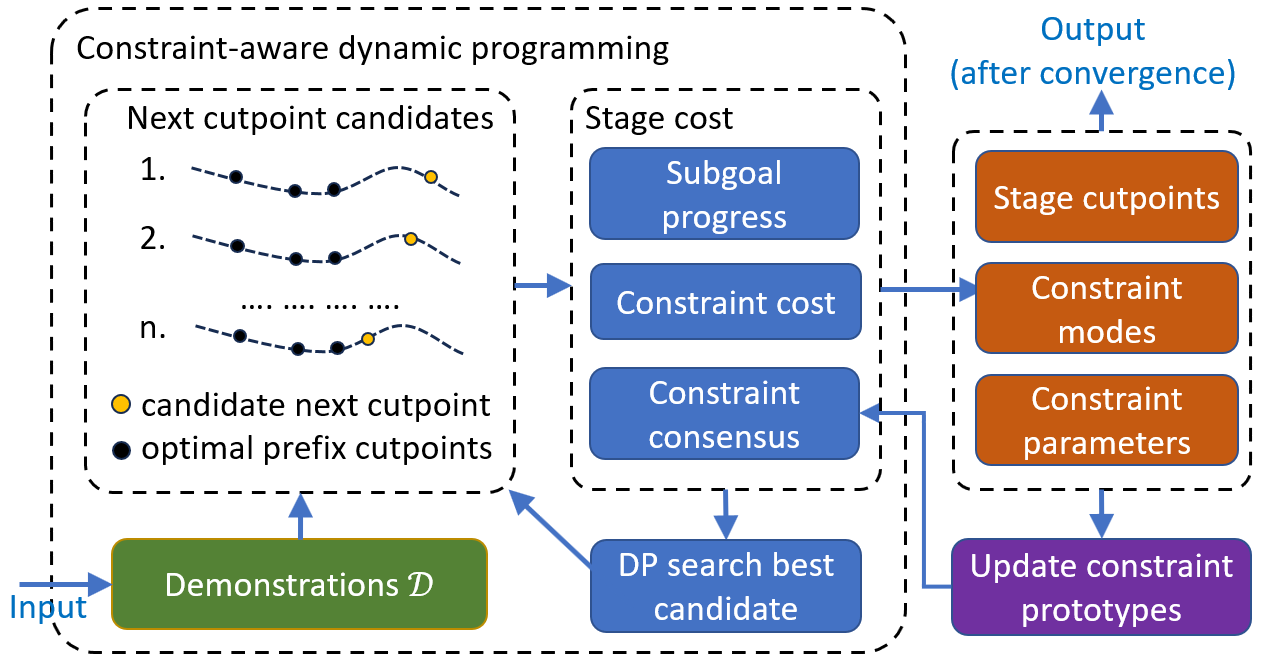
\includegraphics[width=0.49\textwidth]{figs/swcl_block.png}
    \caption{
    Overview of SWCL. Given the current shared constraint prototypes, each demonstration is segmented into $K$ ordered stages by dynamic programming. For every candidate next cutpoint, the corresponding stage interval is evaluated using local feature-constraint evidence, subgoal progress, and cross-demonstration constraint consensus. Dynamic programming selects the cutpoints that minimize the total stage cost. The recovered local constraint modes and parameters are then aggregated across demonstrations to update the shared prototypes. Segmentation and prototype updates alternate until convergence.
    }
    \label{fig:swcl_overview}
\end{figure}


\begin{algorithm}[t]
\caption{Stage-wise Constraint Learning from Demonstrations}
\label{alg:swcl}
\begin{algorithmic}[1]
\Require demonstrations $\mathcal{D}$, number of stages $K$,
feature bank $\Phi$, feature families
$\mathcal{F}_{\mathrm{eq}}$ and $\mathcal{F}_{\mathrm{ineq}}$
\Ensure cutpoints $\{b_k^{(i)}\}$, inferred subgoals
$\{g_k^{(i)}\}$, mode prototype $\hat{\Gamma}$,
and parameter prototypes $\{\hat{\eta}_{k,j}\}$

\State Extract and standardize the feature trajectories
\State Precompute and cache local feature fits and progress costs for all candidate intervals
\State Initialize $\hat{\gamma}_{k,j}=\varnothing$,
$\hat{\eta}_{k,j}=0$, and $q=0$

\Repeat
    \State Set
    $\lambda_{\mathrm{mode}}^{(q)}
    =\rho_q\lambda_{\mathrm{mode}}$
    and
    $\lambda_{\mathrm{par}}^{(q)}
    =\rho_q\lambda_{\mathrm{par}}$,
    with $\rho_0=0$

    \ForAll{demonstrations $i=1,\dots,N$}
        \State Solve the DP recurrence in \eqref{eq:dp_recurrence} using the current prototypes
        \State Backtrack to recover
        $\{\mathcal{I}_k^{(i)}\}_{k=1}^{K}$
        and $\{b_k^{(i)}\}_{k=1}^{K-1}$
        \State Retrieve the corresponding local constraint modes
        $\{\gamma_{k,j}^{(i)}\}$ and parameters $\{\eta_{k,j}^{(i)}\}$
        \State Recover the latent subgoals as
        $g_k^{(i)}=x_{b_k^{(i)}-1}^{(i)}$
    \EndFor

    \State Update $\hat{\Gamma}$ by majority vote over the local modes
    \State Update $\{\hat{\eta}_{k,j}\}$ by median aggregation over mode-consistent active estimates
    \State $q\leftarrow q+1$
\Until{the cutpoints and prototypes converge, or the maximum number of iterations is reached}
\end{algorithmic}
\end{algorithm}


\subsection{Local Feature-constraint Evidence}
\label{subsec:local_constraint_evidence}

We consider an arbitrary demonstration and omit its index throughout this subsection and Section~\ref{subsec:subgoal_progress} for notational clarity. The demonstration index is restored in Section~\ref{subsec:consensus_terms}, where local estimates are compared and aggregated across demonstrations.

For a candidate interval $\mathcal{I}_k$ assigned to stage $k$, SWCL evaluates whether each feature supports an active constraint interpretation. Let $\mathcal{U}_{k,j}=\{\phi_j(x_t):t\in\mathcal{I}_k\}$ denote the samples of feature $j$ within this interval. The local fit determines a constraint mode $\gamma_{k,j}$, an active parameter $\eta_{k,j}$ when applicable, and a feature score used to construct the stage cost. 

\subsubsection{Equality-constrained Features}
An active equality constraint should keep the corresponding feature close to a common stage-specific target. SWCL estimates this target by the segment median $c_{k,j}=\operatorname{median}(\mathcal{U}_{k,j})$ and measures the dispersion around it. To reduce sensitivity to noise and occasional transition samples, only the smallest $\rho$ fraction of absolute deviations are averaged.

Let $a_t=|\phi_j(x_t)-c_{k,j}|$ for $t\in\mathcal{I}_k$, and let $a_{(1)}\leq\cdots\leq a_{(|\mathcal{I}_k|)}$ denote the sorted deviations. The equality score is
\begin{equation}
s_{k,j}^{\mathrm{eq}}
=
\frac{1}{m_\rho}
\sum_{q=1}^{m_\rho} a_{(q)},
\qquad
m_\rho
=
\left\lceil
\rho |\mathcal{I}_k|
\right\rceil .
\label{eq:eq_dispersion_score}
\end{equation}
A small score indicates that most feature samples remain concentrated around a common value and therefore supports an equality constraint. We define the equality evidence margin as $M_{k,j}^{\mathrm{eq}}=[\delta_{\mathrm{eq}}-s_{k,j}^{\mathrm{eq}}]_+$, where $[z]_+=\max(z,0)$ and $\delta_{\mathrm{eq}}$ is a sensitivity parameter. If $M_{k,j}^{\mathrm{eq}}>0$, the local mode and parameter are set to $\gamma_{k,j}=\mathrm{eq}$ and $\eta_{k,j}=c_{k,j}$; otherwise, the feature is treated as inactive, i.e., $\gamma_{k,j}=\varnothing$. We use $\rho=0.8$ by default. 

\subsubsection{Inequality-constrained Features}
We adopt the modeling assumption that, when a one-sided inequality is active and sufficiently expressed in the demonstrations, its feature values exhibit a boundary-anchored distribution: most samples lie on the feasible side of a boundary, with substantial probability mass close to that boundary. This pattern provides evidence for identifying both the activation and direction of the inequality. However, when demonstrations remain well inside the feasible region and rarely approach the true boundary,  the inequality constraints are generally unrecognizable from feasible demonstrations alone~\cite{chou2020local}. In such cases, its activation and direction need to be provided through prior knowledge.

For each candidate interval, SWCL evaluates both candidate directions $d\in\{\mathrm{lb},\mathrm{ub}\}$ using a soft half-Student-$t$ model. The candidate boundary $b_d$ and signed slack $y_d(u)$ are defined as
\begin{equation}
b_d=
\begin{cases}
Q_{q_b}(\mathcal{U}_{k,j}), & d=\mathrm{lb},\\
Q_{1-q_b}(\mathcal{U}_{k,j}), & d=\mathrm{ub},
\end{cases}
\quad
y_d(u)=
\begin{cases}
u-b_d, & d=\mathrm{lb},\\
b_d-u, & d=\mathrm{ub},
\end{cases}
\label{eq:ineq_boundary_slack}
\end{equation}
where $Q_q(\cdot)$ denotes the empirical $q$-quantile and $q_b=0.05$. For either direction, $y_d(u)\geq0$ indicates that the sample lies on the feasible side of the candidate boundary, whereas $y_d(u)<0$ indicates a violation.

The soft half-$t$ density for direction $d$ is
\begin{equation}
p_{\mathrm{ineq}}(u\mid d)
=
\frac{1}{Z}
\begin{cases}
\dfrac{2}{\sigma_d}
t_\nu\!\left(
\dfrac{y_d(u)}{\sigma_d}
\right),
& y_d(u)\geq0,\\[0.9em]
\dfrac{2}{\sigma_d}
t_\nu(0)
\exp\!\left(
\dfrac{y_d(u)}{\kappa\sigma_d}
\right),
& y_d(u)<0,
\end{cases}
\label{eq:soft_half_t_density}
\end{equation}
where $t_\nu$ is the standard Student-$t$ density, $\sigma_d$ describes the feasible-side dispersion\footnote{We use $\nu=3$, for which the normalization constant is $Z=1+2\kappa t_\nu(0)$. Let $\mathcal{Z}_d=\{\max(y_d(u),0):u\in\mathcal{U}_{k,j}\}$ denote the nonnegative clipped slacks. We estimate $\sigma_d=Q_{0.9}(\mathcal{Z}_d)/t_\nu^{-1}(0.95)$ by matching the empirical and modeled $90$th percentiles. For $\nu=3$, $t_3^{-1}(0.95)\approx2.353$.}, and $\kappa$ controls the softness of the infeasible-side tail. The exponential tail permits small noise-induced violations instead of imposing a hard truncation. 

Let $\mathrm{NLL}_{d,k,j}$ denote the average negative log-likelihood under the soft half-$t$ model for direction $d$. SWCL also fits an unconstrained Student-$t$ baseline to the same samples, with average negative log-likelihood $\mathrm{NLL}_{\mathrm{base},k,j}$. The best inequality direction and its relative score are
$d^\star=\arg\min_{d\in\{\mathrm{lb},\mathrm{ub}\}}\mathrm{NLL}_{d,k,j}$
and
$s_{k,j}^{\mathrm{ineq}}
=
\mathrm{NLL}_{d^\star,k,j}
-
\mathrm{NLL}_{\mathrm{base},k,j}$.
The local mode is then determined by
\begin{equation}
\gamma_{k,j}
=
\begin{cases}
d^\star,
& s_{k,j}^{\mathrm{ineq}}<-\delta_{\mathrm{ineq}},\\
\varnothing,
& \text{otherwise}.
\end{cases}
\label{eq:ineq_mode_activation}
\end{equation}
When active, the local constraint parameter is the selected boundary, $\eta_{k,j}=b_{d^\star}$. Otherwise, the feature is treated as locally unconstrained.

\begin{figure}[t]
    \centering
    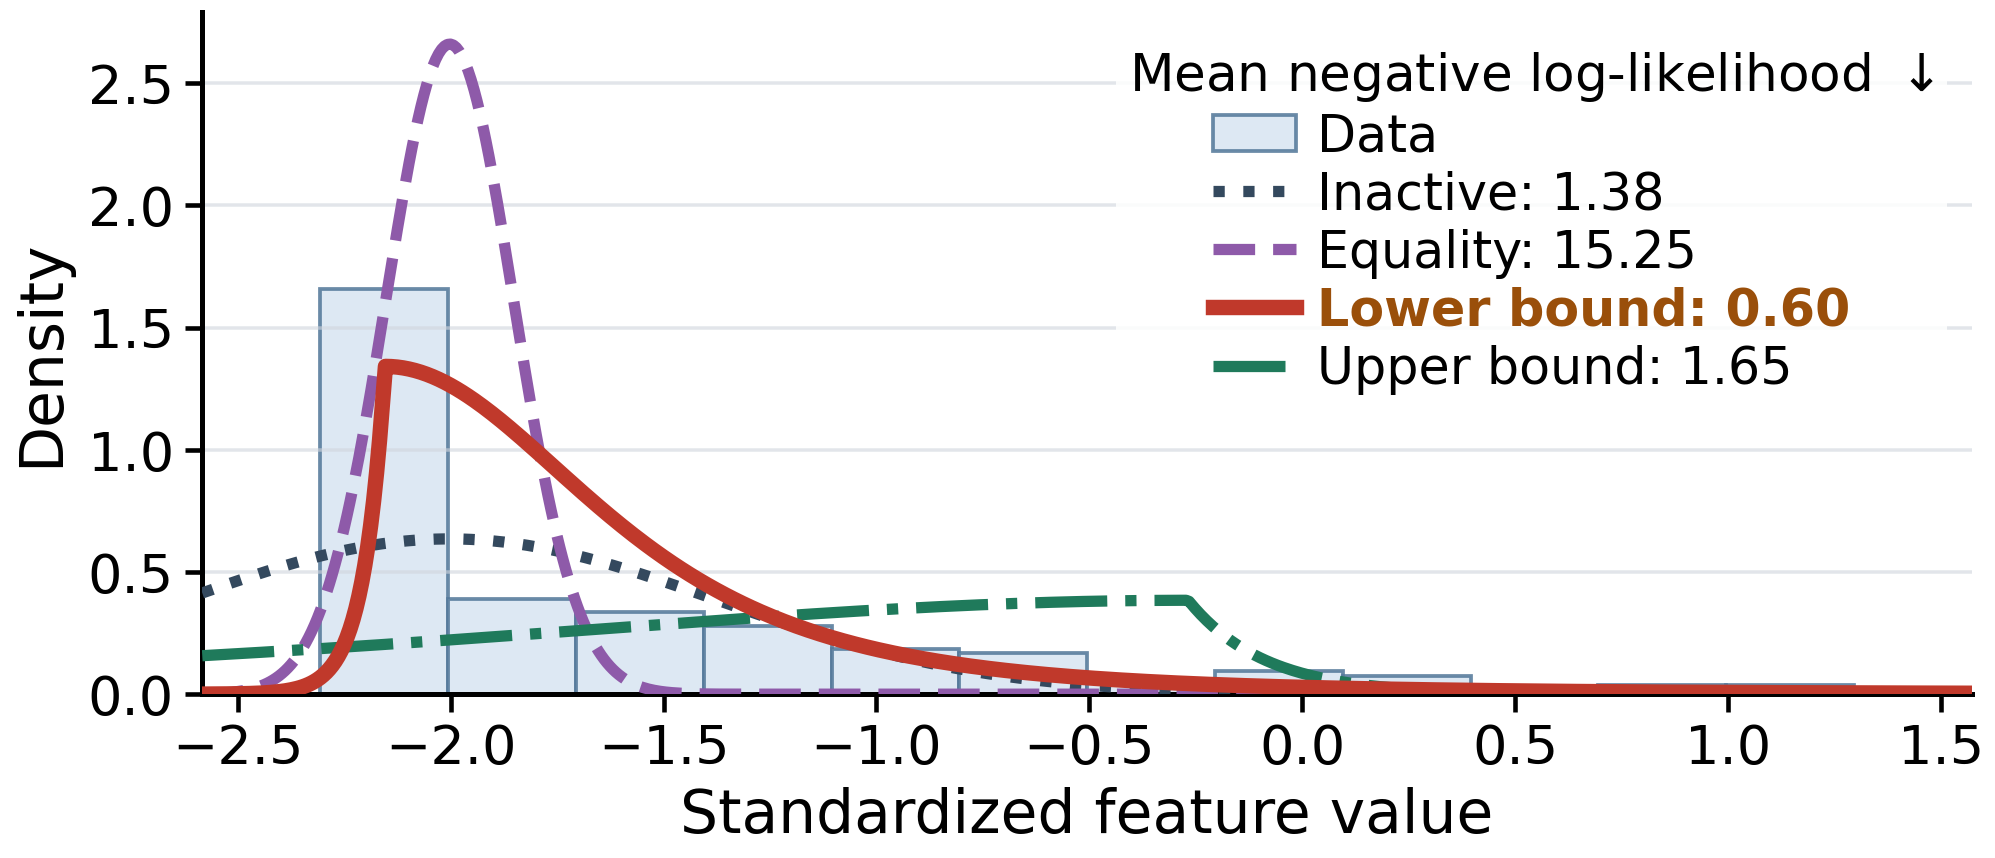
\includegraphics[width=0.85\linewidth]{figs/soft_half_t_example_distribution.png}
    \caption{
    Illustration of the soft half-$t$ inequality model on one candidate interval. The histogram shows the standardized feature samples, the dotted curve shows the unconstrained Student-$t$ baseline, and the red and green curves show the lower- and upper-bound fits. The lower-bound model achieves the lowest average negative log-likelihood and improves sufficiently over the unconstrained baseline; the feature is therefore identified as lower-bound constrained.
    }
    \label{fig:soft_half_t_example}
\end{figure}
Finally, the equality, inequality, and inactive interpretations are converted into a unified feature constraint cost:
\begin{equation}
C_{\mathrm{feat},k,j}
=
\begin{cases}
-\lambda_{\mathrm{eq}}
|\mathcal{I}_k|
M_{k,j}^{\mathrm{eq}},
& \gamma_{k,j}=\mathrm{eq},\\[0.4em]
\lambda_{\mathrm{ineq}}
|\mathcal{I}_k|
\mathrm{NLL}_{d^\star,k,j},
& \gamma_{k,j}\in\{\mathrm{lb},\mathrm{ub}\},\\[0.4em]
0,
& \gamma_{k,j}=\varnothing.
\end{cases}
\label{eq:feature_constraint_contribution}
\end{equation}
The local feature-constraint cost of the candidate stage is then
$C_{\mathrm{feat},k}=\sum_{j=1}^{F}C_{\mathrm{feat},k,j}$.

For equality-constrained features, a larger evidence margin produces a lower cost. For inequality-constrained features, a better one-sided likelihood produces a lower cost, while the unconstrained baseline is used only to decide whether the inequality should be activated. Inactive features contribute zero. 


\subsection{Subgoal Progress}
\label{subsec:subgoal_progress}

Local feature-constraint evidence alone may not define a coherent stage. For example, a long interval can exhibit a consistent feature distribution while containing multiple distinct motions. We therefore introduce a subgoal-progress cost that favors intervals whose states move consistently toward a common endpoint.

The intermediate subgoals are unobserved during learning. A candidate interval $\mathcal{I}_k(s,e)=\{s,\dots,e\}$ jointly proposes a stage boundary and its corresponding subgoal, which is defined by the interval endpoint as $g_k(\mathcal{I}_k)=x_e$. Thus, evaluating progress toward this endpoint also evaluates the subgoal induced by the candidate segmentation.

Let $d_t(\mathcal{I}_k)=\|x_t-g_k(\mathcal{I}_k)\|_2$ denote the distance from state $x_t$ to the candidate subgoal. The progress cost is
\begin{equation}
C_{\mathrm{prog},k}(\mathcal{I}_k)
=
\sum_{t=s}^{e-1}
\operatorname{softplus}_{\beta}
\left(
d_{t+1}(\mathcal{I}_k)
-
d_t(\mathcal{I}_k)
\right),
\label{eq:progress_cost}
\end{equation}
where $\operatorname{softplus}_{\beta}(z)=\beta^{-1}\log(1+\exp(\beta z))$ is a smooth approximation of $[z]_+$. Consequently, a decrease in distance produces a near-zero penalty, whereas motion away from the candidate subgoal is penalized. This term measures stage coherence rather than a constraint to be recovered. Once the cutpoints are inferred, the corresponding intermediate subgoals are obtained directly from the recovered segment endpoints.


\subsection{Cross-demonstration Consensus}
\label{subsec:consensus_terms}

Under our problem formulation, corresponding stages across demonstrations share the same feature-constraint modes and parameters. This shared structure provides additional evidence for resolving the ambiguity of constraint inference: among multiple locally plausible interpretations, SWCL favors those supported consistently by most demonstrations.  

SWCL maintains a shared constraint mode prototype $\hat{\Gamma}=[\hat{\gamma}_{k,j}]$ and parameter prototypes $\{\hat{\eta}_{k,j}\}$. For a fixed segmentation, let $\gamma_{k,j}^{(i)}$ and $\eta_{k,j}^{(i)}$ denote the local mode and parameter estimated from stage interval $\mathcal{I}_k^{(i)}$ of demonstration $i$. The shared mode prototype is obtained by majority vote:
\begin{equation}
\hat{\gamma}_{k,j}
=
\arg\max_{\gamma\in\{\varnothing,\mathrm{eq},\mathrm{lb},\mathrm{ub}\}}
\sum_{i=1}^{N}
\mathds{1}\!\left[
\gamma_{k,j}^{(i)}=\gamma
\right].
\label{eq:mode_consensus_update}
\end{equation}
When $\hat{\gamma}_{k,j}$ is active, its parameter prototype is updated using only demonstrations whose local mode agrees with the shared mode:
\begin{equation}
\hat{\eta}_{k,j}
=
\operatorname{median}
\left\{
\eta_{k,j}^{(i)}
:
\gamma_{k,j}^{(i)}=\hat{\gamma}_{k,j}
\right\},
\qquad
\hat{\gamma}_{k,j}\neq\varnothing.
\label{eq:param_consensus_update}
\end{equation}

During segmentation, a candidate interval $\mathcal{I}$ assigned to stage $k$ in demonstration $i$ is penalized when its local interpretation disagrees with the current shared prototypes. The mode-consensus cost is
\begin{equation}
C_{\mathrm{mode},k}^{(i)}(\mathcal{I})
=
\sum_{j=1}^{F}
\mathds{1}
\left[
\gamma_{k,j}^{(i)}(\mathcal{I})
\neq
\hat{\gamma}_{k,j}
\right],
\label{eq:mode_consensus_cost}
\end{equation}
and the parameter-consensus cost is
\begin{equation}
C_{\mathrm{par},k}^{(i)}(\mathcal{I})
=
\sum_{\substack{
j:\,
\gamma_{k,j}^{(i)}(\mathcal{I})=\hat{\gamma}_{k,j}\\
\hat{\gamma}_{k,j}\neq\varnothing
}}
\left|
\eta_{k,j}^{(i)}(\mathcal{I})
-
\hat{\eta}_{k,j}
\right|.
\label{eq:param_consensus_cost}
\end{equation}
The mode-consensus term encourages agreement on whether each feature is inactive, equality-constrained, lower-bound constrained, or upper-bound constrained. Conditioned on matching active modes, the parameter-consensus term further encourages agreement on the corresponding target or boundary value.

\subsection{Stage Cost and Alternating Dynamic Programming}
\label{subsec:alternating_dp}

For a candidate interval $\mathcal{I}_k^{(i)}$ assigned to stage $k$ in demonstration $i$, SWCL combines local feature-constraint evidence, subgoal progress, and cross-demonstration consensus into the stage cost
\begin{equation}
\begin{aligned}
C_k^{(i)}(\mathcal{I}_k^{(i)})
={}&
C_{\mathrm{feat},k}^{(i)}
+
\lambda_{\mathrm{prog}}C_{\mathrm{prog},k}^{(i)} \\
&+
\lambda_{\mathrm{mode}}C_{\mathrm{mode},k}^{(i)}
+
\lambda_{\mathrm{par}}C_{\mathrm{par},k}^{(i)},
\end{aligned}
\label{eq:full_stage_cost}
\end{equation}
The first two terms evaluate the local constraint interpretation and motion coherence of the interval, while the last two encourage agreement with the shared constraint prototypes.

For a candidate schedule $B^{(i)}$, its total segmentation cost is $\sum_{k=1}^{K}C_k^{(i)}(\mathcal{I}_k^{(i)})$. Conditioned on the current prototypes $\hat{\Gamma}$ and $\{\hat{\eta}_{k,j}\}$, demonstrations are decoupled, and each demonstration can be segmented independently by minimizing this additive cost. We solve the resulting ordered segmentation problem using dynamic programming~\cite{truong2020selective,aminikhanghahi2017survey}.

Let $F_k^{(i)}(t)$ denote the minimum cost of segmenting the prefix $\{x_1^{(i)},\dots,x_t^{(i)}\}$ into the first $k$ stages. Using $[s,t]$ as shorthand for the candidate interval $\{s,\dots,t\}$, the recurrence is
\begin{equation}
F_k^{(i)}(t)
=
\min_{1\leq s\leq t}
\left[
F_{k-1}^{(i)}(s-1)
+
C_k^{(i)}([s,t])
\right].
\label{eq:dp_recurrence}
\end{equation}
The initialization is $F_0^{(i)}(0)=0$ and $F_0^{(i)}(t)=+\infty$ for $t>0$. The minimum full-trajectory cost is $F_K^{(i)}(T_i)$, and the corresponding cutpoints are recovered by backtracking. Conditioned on the current prototypes, this DP step searches over all ordered cutpoint sequences and exactly solves the segmentation subproblem.

The segmentation and prototype estimates depend on each other: the consensus costs require shared prototypes, while the prototypes are estimated from the recovered stage intervals. SWCL therefore alternates between DP segmentation and prototype aggregation. The first pass uses zero consensus weights and is determined only by local feature evidence and subgoal progress. In subsequent iterations, the consensus weights are gradually introduced using $\lambda_{\mathrm{mode}}^{(q)}=\rho_q\lambda_{\mathrm{mode}}$ and $\lambda_{\mathrm{par}}^{(q)}=\rho_q\lambda_{\mathrm{par}}$, where $\rho_q$ increases from zero toward one linearly. This prevents unreliable initial prototypes from dominating the segmentation while progressively enforcing cross-demonstration agreement.

The complete procedure is summarized in Algorithm~\ref{alg:swcl}.

The local feature fits and subgoal-progress costs depend only on the demonstration and candidate interval, not on the shared prototypes. They are therefore computed once and cached before alternating learning. At each iteration, only the prototype-dependent mode- and parameter-consensus costs are recomputed. Cache construction is independent across demonstrations and candidate intervals and can be parallelized.

\section{Simulation Experiment}
\label{sec:experiment}

\subsection{Experimental Setup}
\label{subsec:exp_setup}

\subsubsection{Benchmark Datasets}

We evaluate SWCL on three simulated multi-stage benchmark tasks: \texttt{S3ObsAvoid}, \texttt{S4SlideInsert}, and \texttt{S5SphereInspect} with three baselines. The tasks contain three, four, and five ordered stages, respectively, and are designed to evaluate stage-wise constraint-mode identification, and constraint-parameter estimation.

\textbf{S3ObsAvoid.} A three-stage planar navigation task: obstacle avoidance $\rightarrow$ transition $\rightarrow$ terminal arc following.
Fig.~\ref{fig:s3_demo_cutpoints} shows a representative demonstration and its ground-truth stage cutpoints.

\begin{figure}[t]
    \centering
    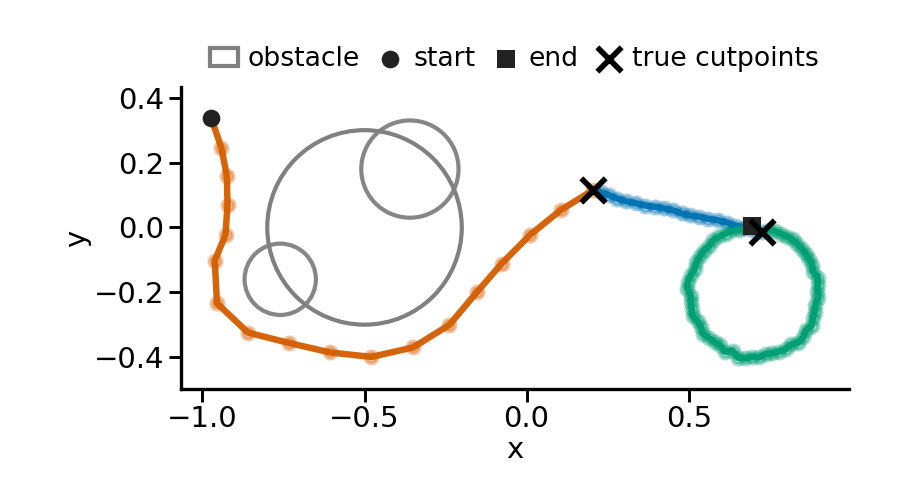
\includegraphics[width=0.83\linewidth]{figs/s3_demonstration.png}
    \caption{
    Example demonstration from the \texttt{S3ObsAvoid} environment. 
    The colored trajectory segments correspond to the three ground-truth stages: obstacle avoidance, transition, and terminal arc following. 
    Gray ellipses denote the composite obstacle, the black circle and square mark the start and end states, and black crosses indicate the true stage cutpoints.
    }
    \label{fig:s3_demo_cutpoints}
\end{figure}

\textbf{S4SlideInsert.} A four-stage slide-and-insert task: free-space approach $\rightarrow$ surface contact and alignment $\rightarrow$ guided sliding $\rightarrow$ final insertion.
The task is performed by a UR5 arm simulated in PyBullet.

\textbf{S5SphereInspect.} A five-stage spherical inspection task: approach $\rightarrow$ surface inspection $\rightarrow$ transition $\rightarrow$ outer-shell inspection $\rightarrow$ departure.
The task is also performed by a simulated UR5 arm, and Fig.~\ref{fig:s5_planning_snapshots} visualizes its five stages.

The feature banks of the three tasks are summarized in Table~\ref{tab:dataset_features}, while their ground-truth and learned stage-wise constraints are compared in Fig.~\ref{fig:true_learned_modes_all}. Only a subset of the exposed features is constrained in each stage; the remaining features are included to evaluate whether the method can correctly identify inactive or decoy features. All methods are trained on the same
$10$ demonstrations per task, generated as feasible planned trajectories satisfying the task structure in
\eqref{eq:stagewise_feasibility_problem}. All code and datasets are available at
\url{https://github.com/epfl-lasa/Constraints_Learning_Learn_Stage-wise_Constraints_from_Demonstrations}.



% \begin{table*}[t]
% \centering
% \footnotesize
% \setlength{\tabcolsep}{2.2pt}
% \renewcommand{\arraystretch}{1.03}
% \newcommand{\val}[1]{\mbox{#1}}
% \begin{tabular}{
% >{\raggedright\arraybackslash}p{1.95cm}
% >{\raggedright\arraybackslash}p{2.35cm}
% >{\raggedright\arraybackslash}p{6.85cm}
% *{5}{>{\centering\arraybackslash}p{0.85cm}}
% }
% \toprule
% Dataset & Feature & Description & stage 1 & stage 2 & stage 3 & stage 4 & stage 5 \\
% \midrule

% \multirow{6}{1.85cm}{\centering\textbf{S3ObsAvoid}}
% & \texttt{obs\_dist}  & Distance to the obstacle (cm) & \val{$\geq 40.0$} & \NoAct & \NoAct & \NA & \NA \\
% & \texttt{speed}      & Speed magnitude (cm/s) & \NoAct & \val{$=5.5$} & \val{$=4.5$} & \NA & \NA \\
% & \texttt{arc\_dist}  & Distance to the terminal circle center (cm) & \NoAct & \NoAct & \val{$=20.0$} & \NA & \NA \\
% & \texttt{heading}    & Heading angle (rad) & \NoAct & \NoAct & \NoAct & \NA & \NA \\
% & \texttt{line\_dist} & Distance to an irrelevant straight line (cm) & \NoAct & \NoAct & \NoAct & \NA & \NA \\
% & \texttt{noise}      & Sine noise (unitless) & \NoAct & \NoAct & \NoAct & \NA & \NA \\

% \addlinespace[0.22em]
% \midrule
% \addlinespace[0.02em]

% \multirow{7}{1.85cm}{\centering\textbf{S4SlideInsert}}
% & \texttt{surf\_dist}    & Distance to the table contact surface (mm) & \NoAct & \val{$=0$} & \val{$=0$} & \val{$=0$} & \NA \\
% & \texttt{center\_dist}  & Absolute lateral distance from the slot centerline (mm) & \NoAct & \val{$=0$} & \val{$=0$} & \val{$=0$} & \NA \\
% & \texttt{orient\_err}   & Absolute orientation error relative to the slot (deg) & \NoAct & \NoAct & \val{$\leq 3.44$} & \val{$\leq 2.29$} & \NA \\
% & \texttt{speed}         & Speed magnitude of the tool (mm/s) & \NoAct & \NoAct & \val{$\leq 7.20$} & \val{$\leq 2.88$} & \NA \\
% & \texttt{normal\_force} & Normal contact force applied against the guide (N) & \NoAct & \val{$\geq 4.0$} & \val{$\geq 7.2$} & \val{$\geq 10.0$} & \NA \\
% & \texttt{start\_dist}   & Distance to the demonstration start pose (mm) & \NoAct & \NoAct & \NoAct & \NoAct & \NA \\
% & \texttt{insert\_err}   & Remaining insertion distance along the slot (mm) & \NoAct & \NoAct & \NoAct & \NoAct & \NA \\

% \addlinespace[0.22em]
% \midrule
% \addlinespace[0.02em]

% \multirow{6}{1.85cm}{\centering\textbf{S5SphereInspect}}
% & \texttt{surf\_dist}  & Radial distance to the sphere surface (mm) & \NoAct & \val{$=0$} & \NoAct & \val{$=32.4$} & \NoAct \\
% & \texttt{normal\_err} & Angle between the tool axis and sphere normal (deg) & \NoAct & \val{$\leq 2.29$} & \NoAct & \NoAct & \NoAct \\
% & \texttt{speed}       & Speed magnitude of the tool (mm/s) & \NoAct & \val{$\leq 8.46$} & \NoAct & \val{$\leq 8.46$} & \NoAct \\
% & \texttt{ang\_speed}  & Angular speed magnitude (deg/s) & \NoAct & \NoAct & \NoAct & \NoAct & \NoAct \\
% & \texttt{start\_dist} & Distance to the demonstration start position (mm) & \NoAct & \NoAct & \NoAct & \NoAct & \NoAct \\
% & \texttt{goal\_dist}  & Distance to the nominal inspection goal (mm) & \NoAct & \NoAct & \NoAct & \NoAct & \NoAct \\
% \bottomrule
% \end{tabular}
% \vspace{2pt}

% \caption{Features and true stage-wise constraint values. \NoAct indicates an unconstrained feature-stage pair, and gray block indicates stages not present in that dataset.}
% \label{tab:dataset_features}
% \end{table*}


\begin{table}[t]
\centering
\footnotesize
\setlength{\tabcolsep}{3pt}
\renewcommand{\arraystretch}{1.05}

\begin{tabularx}{\columnwidth}{
@{}
>{\raggedright\arraybackslash}p{2.05cm}
>{\raggedright\arraybackslash}X
>{\centering\arraybackslash}p{0.75cm}
@{}
}
\toprule
Feature & Description & Unit \\
\midrule

\multicolumn{3}{@{}l}{\textbf{\texttt{S3ObsAvoid}}} \\
\addlinespace[0.1em]
\texttt{obs\_dist}
& Distance to the obstacle
& cm \\

\texttt{speed}
& Speed magnitude
& cm/s \\

\texttt{arc\_dist}
& Distance to the terminal-circle center
& cm \\

\texttt{heading}
& Heading angle
& rad \\

\texttt{line\_dist}
& Distance to an irrelevant straight line
& cm \\

\texttt{noise}
& Sine noise
& -- \\

\addlinespace[0.25em]
\midrule
\addlinespace[0.1em]

\multicolumn{3}{@{}l}{\textbf{\texttt{S4SlideInsert}}} \\
\addlinespace[0.1em]
\texttt{surf\_dist}
& Distance to the table contact surface
& mm \\

\texttt{center\_dist}
& Absolute lateral distance from the slot centerline
& mm \\

\texttt{orient\_err}
& Absolute orientation error relative to the slot
& deg \\

\texttt{speed}
& Speed magnitude of the tool
& mm/s \\

\texttt{normal\_force}
& Normal contact force applied against the guide
& N \\

\texttt{start\_dist}
& Distance to the demonstration start pose
& mm \\

\texttt{insert\_err}
& Remaining insertion distance along the slot
& mm \\

\addlinespace[0.25em]
\midrule
\addlinespace[0.1em]

\multicolumn{3}{@{}l}{\textbf{\texttt{S5SphereInspect}}} \\
\addlinespace[0.1em]
\texttt{surf\_dist}
& Radial distance to the sphere surface
& mm \\

\texttt{normal\_err}
& Angle between the tool axis and the sphere normal
& deg \\

\texttt{speed}
& Speed magnitude of the tool
& mm/s \\

\texttt{ang\_speed}
& Angular speed magnitude
& deg/s \\

\texttt{start\_dist}
& Distance to the demonstration start position
& mm \\

\texttt{goal\_dist}
& Distance to the nominal inspection goal
& mm \\

\bottomrule
\end{tabularx}

\caption{
Feature banks used in the three benchmark tasks.
Units refer to the feature values before standardization.
}
\label{tab:dataset_features}
\end{table}

\subsubsection{Baselines}
As discussed in the related work section, most existing constraint-learning methods are not designed to recover multi-stage constraints directly. Therefore, we adapt three representative segmentation paradigms to the stage-wise constraint learning setting.

It is important to note that these baselines do not explicitly recover the full constraint mode matrix $\Gamma$. In particular, they are not designed to determine which stage-feature pairs are active or inactive. Therefore, when computing constraint-parameter errors for the baselines, we provide the ground-truth active stage-feature pairs and compare only the parameters fitted on those pairs. For inequality-type features, the ground-truth lower/upper direction is also provided during parameter extraction. This protocol is favorable to the baselines, since SWCL must infer both the active pairs and the inequality directions automatically.

\textbf{Feature-constrained Hidden Markov Model (FCHMM).}
This baseline is adapted from the classical Gaussian-emission HMM segmentation pipeline~\cite{rabiner1989hmm}. We adapt it to perform segmentation and constraint modeling jointly. Specifically, each latent stage is augmented with explicit feature-wise constraint emissions. For equality-type features, the emission is modeled by a Student-\(t\) distribution, whose fitted center is extracted as the learned equality parameter. For inequality-type features, we use the same soft half-\(t\) local fitting rule as SWCL, but with the ground-truth inequality direction provided. The fitted boundary is extracted as the learned inequality parameter.

\textbf{Autoregressive Hidden Semi-Markov Model (ARHSMM).}
This baseline first segments the demonstrations using an autoregressive hidden semi-Markov model~\cite{johnson2013hsmm}, where the autoregressive observation model is fitted on the joint state-feature representation $(x_t,\phi(x_t))$. After segmentation, it performs a post-hoc constraint-parameter fitting step on the recovered segments using the ground-truth active stage-feature pairs. For equality-type features, the parameter is estimated by the segment median. For inequality-type features, the boundary is estimated from the corresponding tail quantile using the ground-truth lower/upper direction. It therefore represents a \emph{segmentation-first, constraint-fitting-second} pipeline, which contrasts with the joint learning pipeline of SWCL and FCHMM.

\textbf{Ordered clustering (Cluster).}
This baseline segments demonstrations by ordered clustering in the joint state-feature space, following the general idea of clustering-based trajectory segmentation~\cite{keogh2004segmenting}. After segmentation, it fits stage-wise constraint parameters on the recovered segments using the same post-hoc fitting protocol as ARHSMM. 

\subsubsection{Evaluation metrics}
We evaluate the four methods mainly on constraint recovery quality and secondly on segmentation quality.

\textbf{Normalized constraint error.}
For each truly active stage-feature pair, we compare the learned constraint parameter against the ground-truth target or boundary value. Since different features have different physical scales, the absolute error is normalized by a feature-specific scale estimated from the demonstrations and averaged across all truly constrained stage-feature pairs. Lower values indicate more accurate constraint recovery. Truly inactive stage-feature pairs are excluded from this metric. For SWCL, we additionally inspect the learned constraint mode matrix and the corresponding recovered parameter values. While the other three baselines directly use ground truth constraint mode and only compare constraint values. 

\textbf{Mean absolute cutpoint error.}
For each demonstration, we compare each predicted stage cutpoint with the corresponding ground-truth cutpoint and compute the absolute boundary error. We first average these errors over all cutpoints within the same demonstration, and then average the resulting per-demonstration errors over all demonstrations. Lower values indicate more accurate segmentation.

\subsection{Results}
\subsubsection{Main benchmark comparison}
\label{subsec:main_benchmark}

Figure~\ref{fig:benchmark_main} compares SWCL with the three baselines on the benchmark datasets. The top row reports mean absolute cutpoint error and the bottom row reports normalized constraint error. The three baselines are trained from $10$ random initializations and the reported results are averaged across these runs. In contrast, SWCL is run once, since it does not depend on random initialization. The parameters of SWCL and the baselines are tuned by sweeping.

SWCL achieves the lowest error on both metrics across all three datasets. In terms of segmentation, SWCL recovers substantially more accurate cutpoints than the baselines, especially on \texttt{S3ObsAvoid} and \texttt{S5SphereInspect}. The advantage is also reflected in constraint recovery: SWCL obtains the lowest normalized constraint error in all tasks, with the largest gap appearing on \texttt{S5SphereInspect}, where the baselines struggle to recover the correct stage-wise constraint values. Fig.~\ref{fig:s5_feature_profile} shows the normalized feature profiles of one \texttt{S5SphereInspect} demonstration together with the SWCL-learned and ground-truth cutpoints. The learned cutpoints are close to the true stage cutpoints and align with visible changes in the feature regimes. 

\begin{figure}[t]
    \centering
    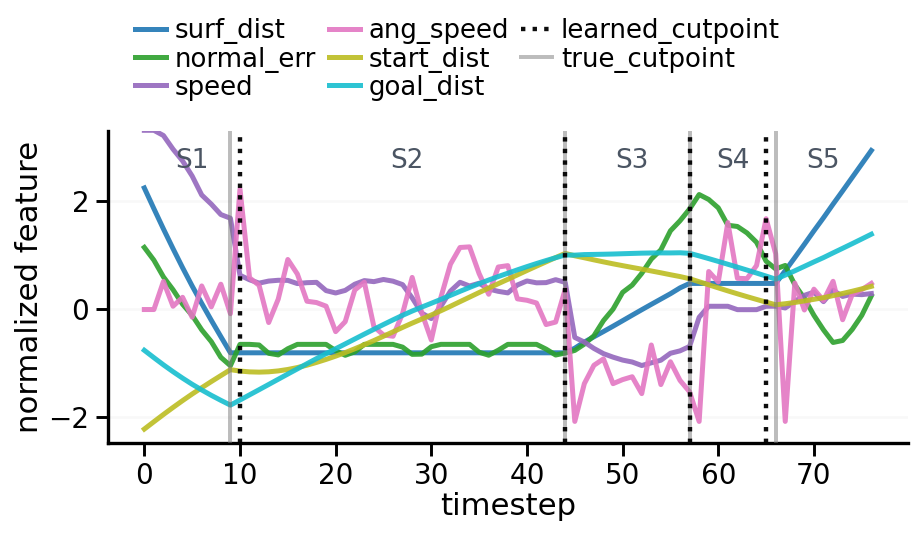
\includegraphics[width=0.8\linewidth]{figs/s5_feature_profile.png}
    \caption{
    Normalized feature profiles of one representative \texttt{S5SphereInspect} demonstration. 
    Solid gray vertical lines indicate the ground-truth cutpoints, and dotted black vertical lines indicate the cutpoints learned by SWCL. 
    }
    \label{fig:s5_feature_profile}
\end{figure}

Among the baselines, none performs consistently well across both metrics and all datasets. FCHMM sometimes achieves reasonable segmentation accuracy, but its constraint error remains higher than SWCL, especially on \texttt{S5SphereInspect}. ARHSMM generally gives larger cutpoint errors and also has relatively high constraint error, suggesting that segmentation based mainly on autoregressive temporal structure does not align well with the constraint-relevant stages in these tasks. Cluster obtains competitive cutpoint error on some datasets, but its constraint recovery remains less accurate than SWCL because the constraint parameters are fitted only after segmentation.

A second visible pattern is variance. ARHSMM and FCHMM exhibit large error bars on several datasets, indicating substantial sensitivity to random initialization or unstable segmentation. By contrast, SWCL has much smaller variability because each segmentation update is solved by a full dynamic-programming search conditioned on the current shared prototypes. These results support a major benefit of SWCL: coupling local constraint evidence, subgoal progress, and cross-demonstration consensus leads to more reliable recovery of both stage cutpoints and stage-wise constraints.

\begin{figure}[t]
    \centering
    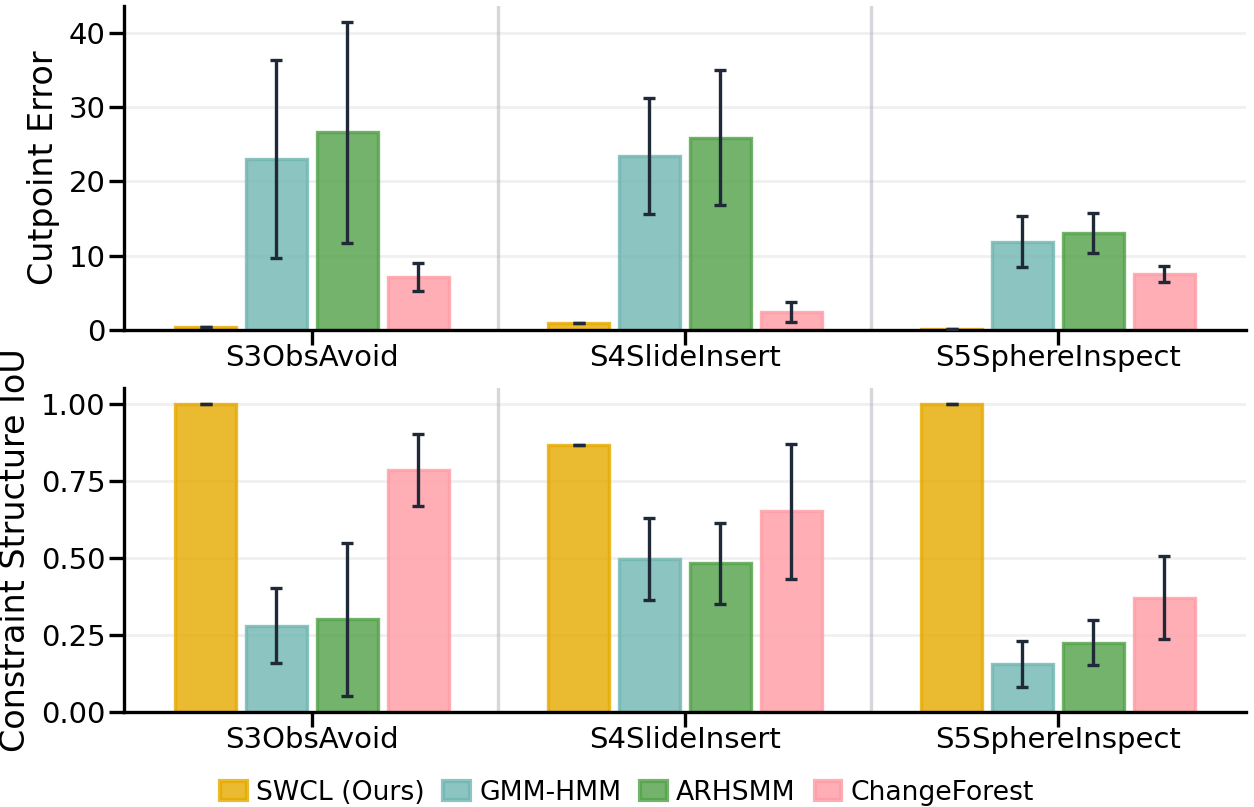
\includegraphics[width=0.9\linewidth]{figs/benchmark_results_comparison.png}
    \caption{Main benchmark comparison across the three datasets. Top: mean absolute cutpoint error. Bottom: normalized constraint error. Lower is better in both plots.}
    \label{fig:benchmark_main}
\end{figure}


% \begin{figure*}[t]
%     \centering
%     \makebox[\textwidth][c]{%
%     \subfloat[\texttt{S3ObsAvoid}]{
%         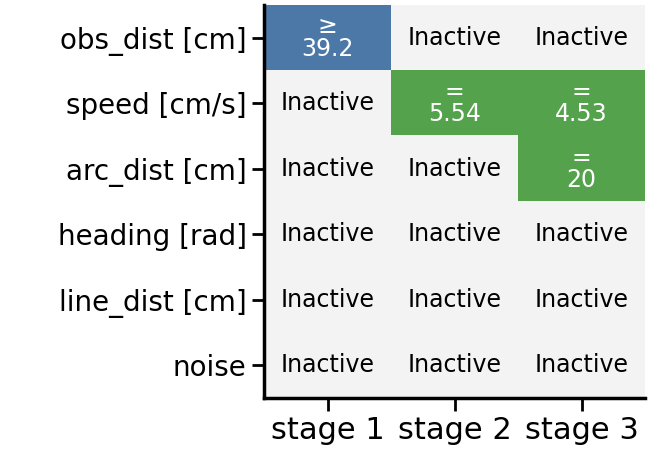
\includegraphics[height=0.142\textheight]{figs/s3_learned_constraint.png}
%     }\hspace{0.00\textwidth}%
%     \subfloat[\texttt{S4SlideInsert}]{
%         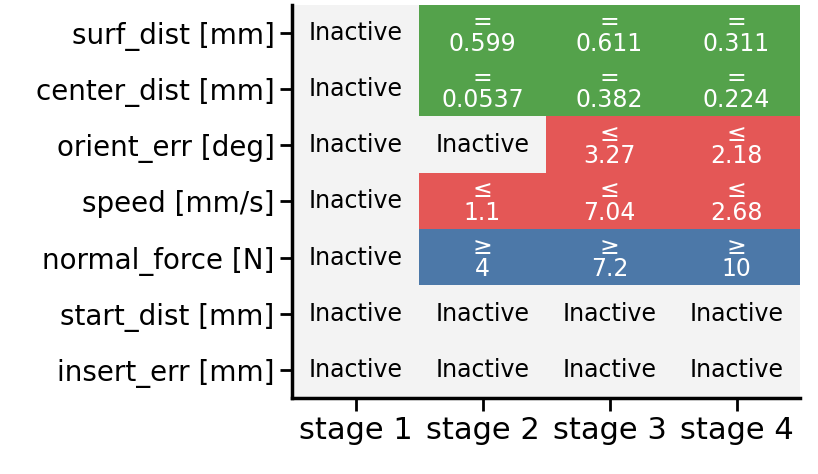
\includegraphics[height=0.142\textheight]{figs/s4_learned_constraint.png}
%     }\hspace{0.00\textwidth}%
%     \subfloat[\texttt{S5SphereInspect}]{
%         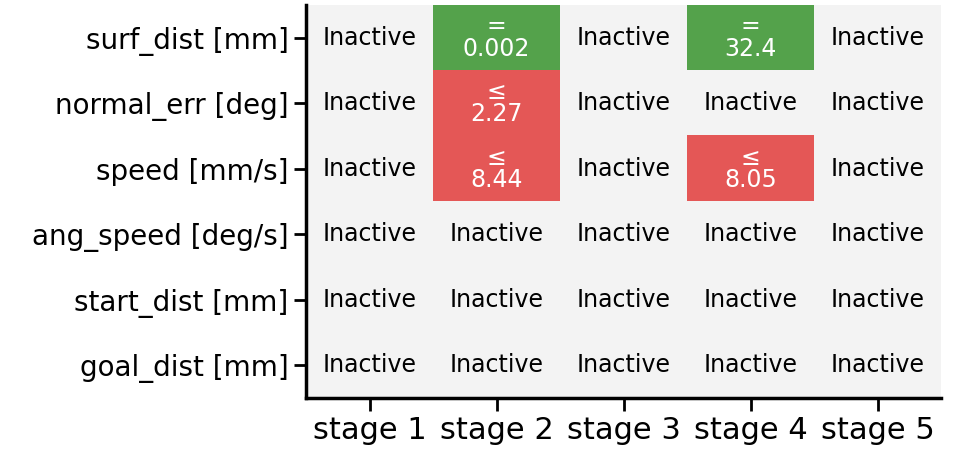
\includegraphics[height=0.142\textheight]{figs/s5_learned_constraint.png}
%     }}
%     \caption{Learned stage-wise constraint matrices for SWCL. Each cell corresponds to one stage-feature pair. Colors indicate the learned mode. For active constraint entries, the cell text reports the learned constraint form and its estimated constraint value.}
%     \label{fig:learned_modes_all}
% \end{figure*}
\begin{figure*}[t]
    \centering
    \subfloat[\texttt{S3ObsAvoid}\label{fig:constraints_s3}]{
        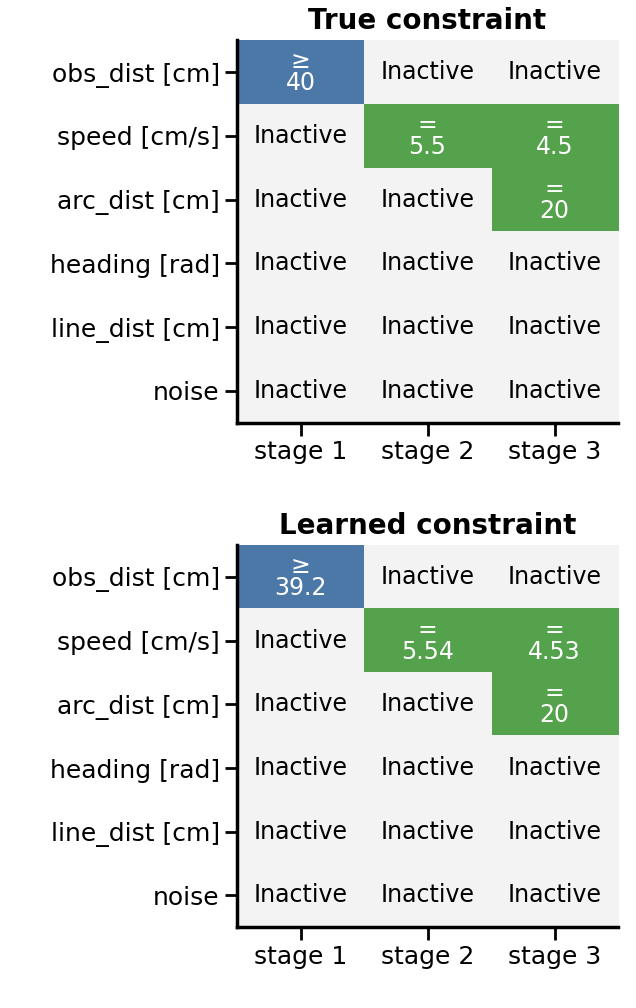
\includegraphics[height=0.3\textheight]
        {figs/S3ObsAvoid_true_vs_learned_constraints.png}
    }
    \hfill
    \subfloat[\texttt{S4SlideInsert}\label{fig:constraints_s4}]{
        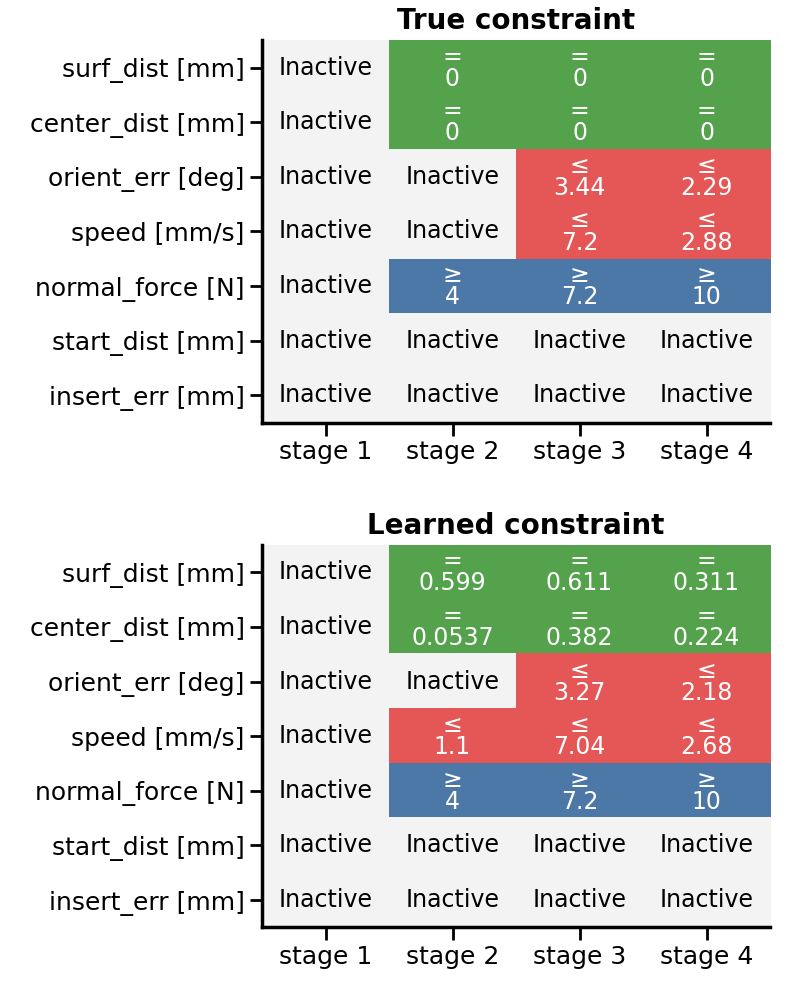
\includegraphics[height=0.3\textheight]
        {figs/S4SlideInsert_true_vs_learned_constraints.png}
    }
    \hfill
    \subfloat[\texttt{S5SphereInspect}\label{fig:constraints_s5}]{
        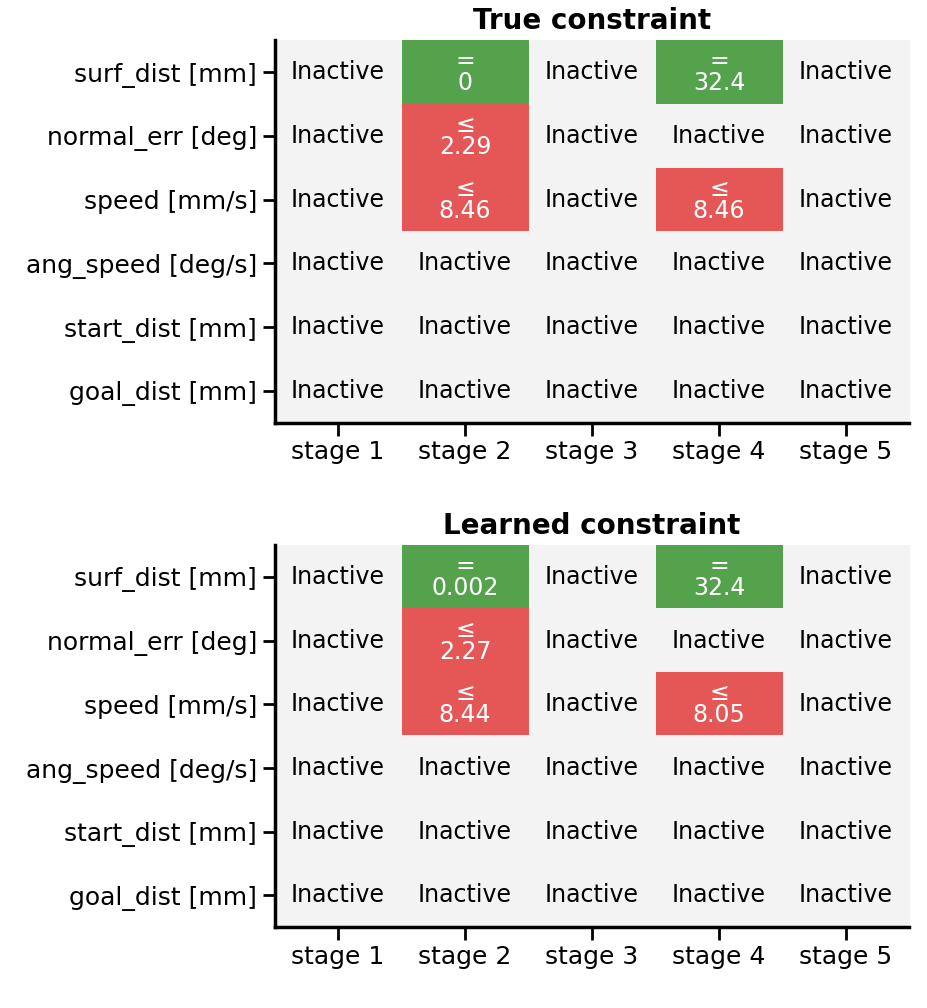
\includegraphics[height=0.3\textheight]
        {figs/S5SphereInspect_true_vs_learned_constraints.png}
    }
    \caption[Ground-truth and learned stage-wise constraints.]{
    Comparison of the ground-truth and learned stage-wise constraint
    matrices for the three benchmark tasks. In each panel, the upper
    matrix shows the ground-truth constraints and the lower matrix shows
    the constraints recovered by SWCL. Each cell corresponds to one
    stage-feature pair. Colors indicate the constraint mode, while the
    cell text reports the equality target or inequality boundary in the
    physical units shown on the vertical axis. Inactive entries indicate
    unconstrained stage-feature pairs.
    }
    \label{fig:true_learned_modes_all}
\end{figure*}

\begin{figure}[t]
    \centering
    \subfloat[Tilted surface transfer\label{fig:s4_transfer_tilt}]{
        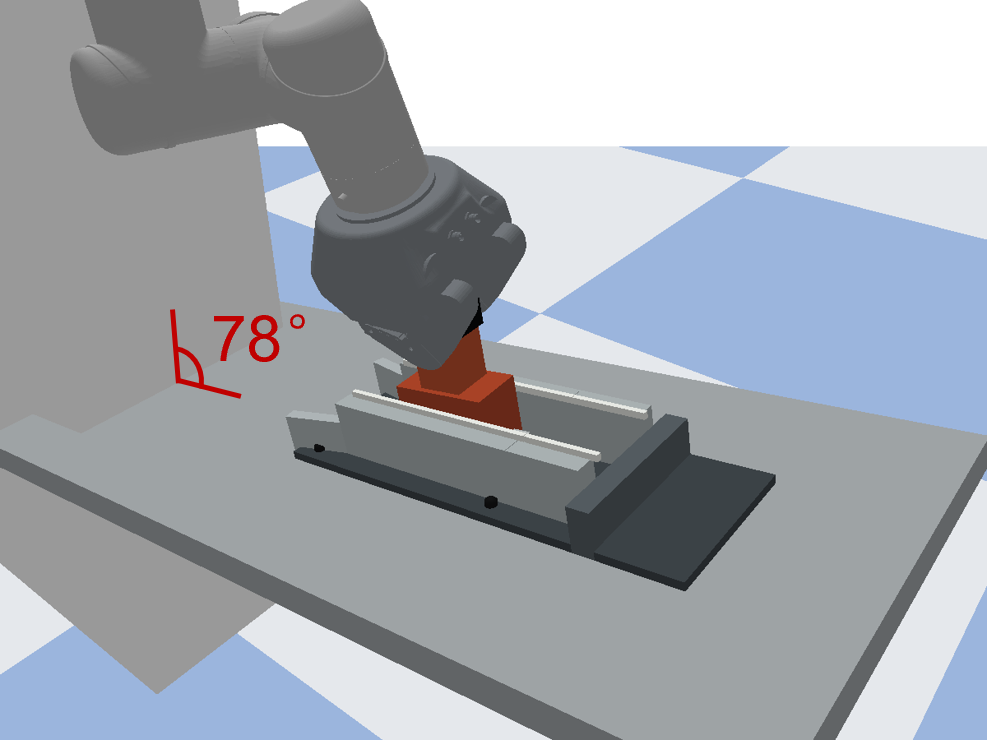
\includegraphics[width=0.49\linewidth]{figs/s4_transfer_tilt.png}
    }
    \subfloat[Curved rail transfer\label{fig:s4_transfer_curve}]{
        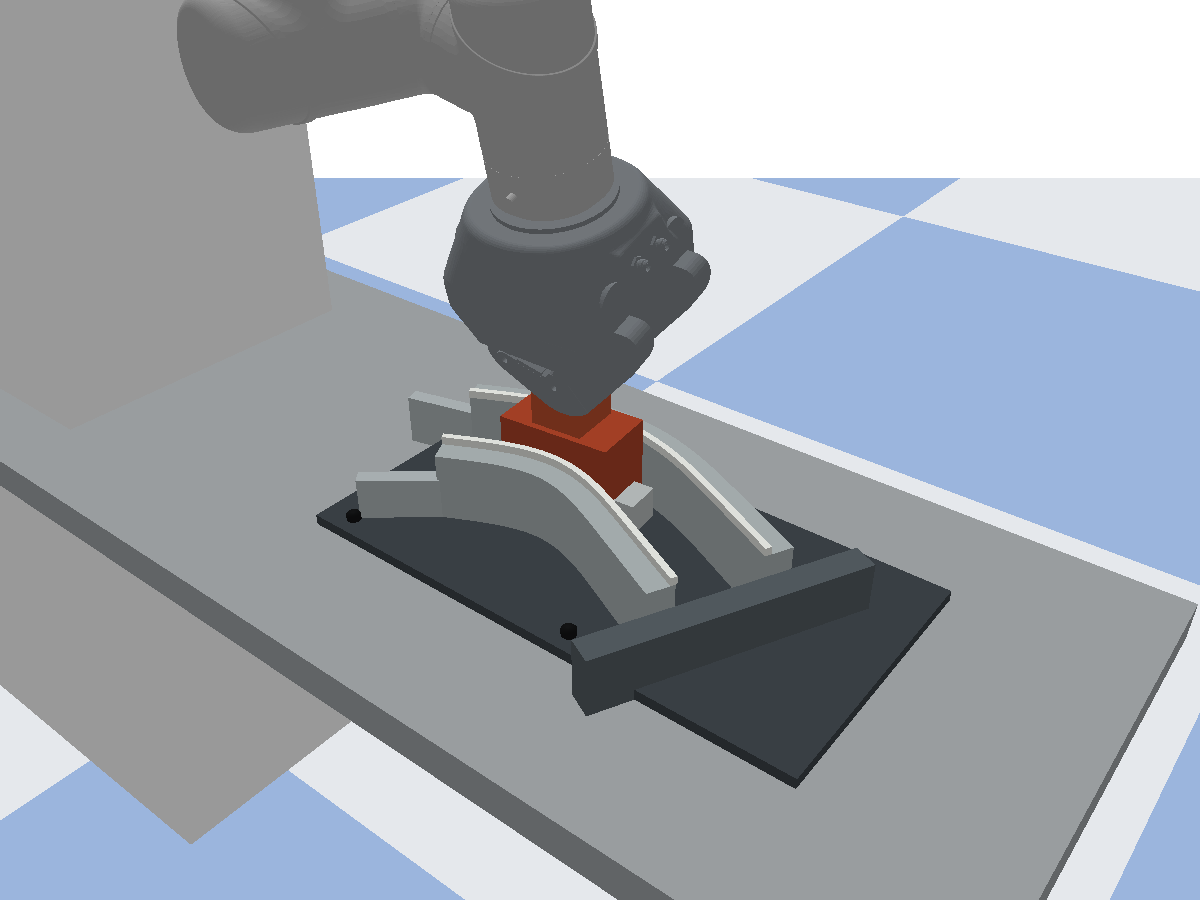
\includegraphics[width=0.49\linewidth]{figs/s4_transfer_curve.png}
    }
    \caption{
    Transfer of learned \texttt{S4SlideInsert} constraints to two modified tasks with the same stage-wise constraint semantics but different environments.
    (a) The guide surface is tilted.
    (b) The straight guide is replaced by a curved rail.
    }
    \label{fig:s4_transfer}
\end{figure}

\begin{figure*}[t]
    \centering
    \subfloat[stage 1: approach]{
        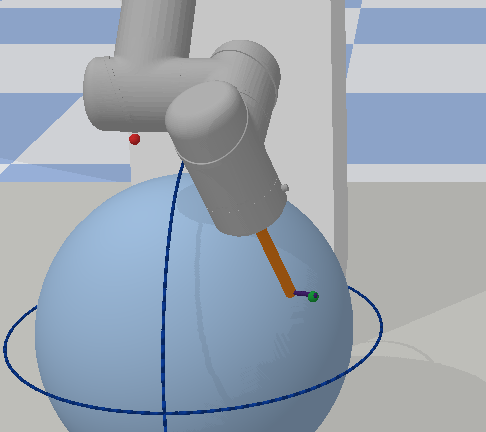
\includegraphics[width=0.178\textwidth]{figs/s5_planned_frame_000010.png}
    }\hspace{0.002\textwidth}
    \subfloat[stage 2: surface inspection]{
        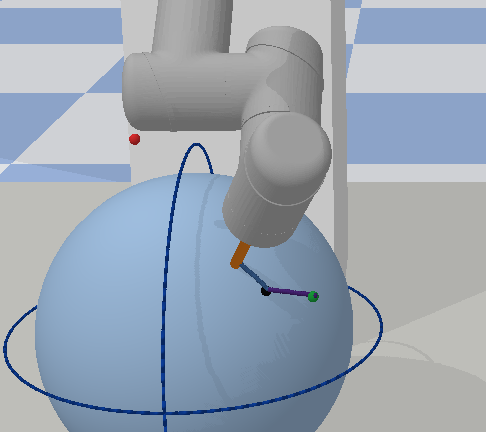
\includegraphics[width=0.178\textwidth]{figs/s5_planned_frame_000050.png}
    }\hspace{0.002\textwidth}
    \subfloat[stage 3: transition]{
        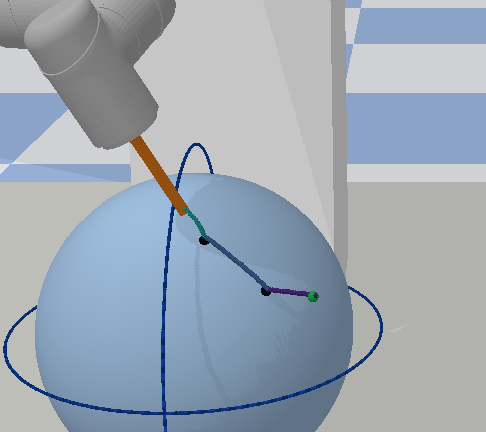
\includegraphics[width=0.178\textwidth]{figs/s5_planned_frame_000090.png}
    }\hspace{0.002\textwidth}
    \subfloat[stage 4: outer-shell inspection]{
        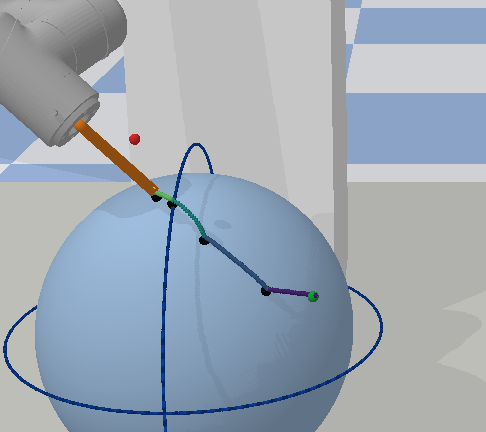
\includegraphics[width=0.178\textwidth]{figs/s5_planned_frame_000115.png}
    }\hspace{0.002\textwidth}
    \subfloat[stage 5: departure]{
        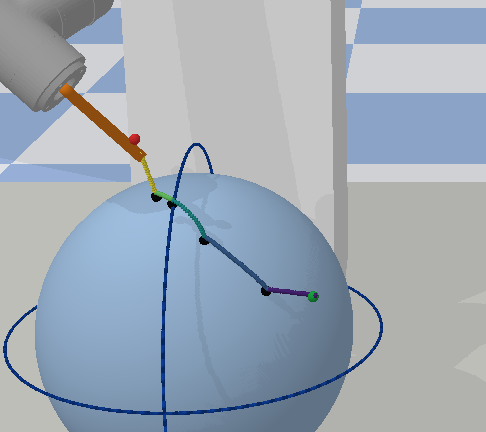
\includegraphics[width=0.178\textwidth]{figs/s5_planned_frame_000130.png}
    }
    \caption{
    PyBullet execution snapshots of a new \texttt{S5SphereInspect} planning instance using the learned stage-wise constraints. 
    The five snapshots correspond to the five stages of the task: 
    (a) the tool approaches the sphere from a new start configuration; 
    (b) it performs surface inspection while maintaining the learned surface-distance, normal-alignment, and speed constraints; 
    (c) it transitions away from the strongly constrained surface-tracing regime; 
    (d) it performs inspection on a larger spherical shell farther from the sphere; 
    and (e) it departs toward the terminal goal.
    }
    \label{fig:s5_planning_snapshots}
\end{figure*}

\subsubsection{Learned constraint modes of SWCL}

Beyond the scalar error metrics, we directly examine the stage-wise constraint structure recovered by SWCL. Fig.~\ref{fig:true_learned_modes_all} compares the ground-truth constraint matrix with the learned shared matrix $\hat{\Gamma}=[\hat{\gamma}_{k,j}]$ for each benchmark task. Each cell represents one stage-feature pair and is labeled as inactive, equality-constrained, lower-bound constrained, or upper-bound constrained. For active entries, the cell text additionally reports the corresponding equality target or inequality boundary in the physical unit shown on the vertical axis. 

SWCL recovers the correct full constraint-mode structure on \texttt{S3ObsAvoid} and \texttt{S5SphereInspect}. On \texttt{S4SlideInsert}, most modes are also recovered correctly. The main mismatch is that SWCL additionally identifies a speed upper-bound constraint in stage 2, where the ground-truth mode is inactive. This likely occurs because the motion slows down from stage 1 to stage 2, making the local speed profile appear one-sided to be interpreted as an active inequality constraint. Overall, the learned constraint matrices show that SWCL recovers the dominant task-level constraint structure, while also producing interpretable numerical constraint values for the active stage-feature pairs.

\subsection{Reuse the Learned Constraints for Planning}
\label{subsec:planning_learned_constraints}
We further evaluate whether the learned stage-wise constraints can be reused for planning. Given the learned constraint mode prototype $\hat\Gamma$ and parameter prototypes $\{\hat\eta_{k,j}\}$, we construct new task instances with prescribed start states, final goals, and trajectory lengths, and use the learned active constraints as stage-wise feasibility conditions in \eqref{eq:stagewise_feasibility_problem}. Different from the formulation in \eqref{eq:stagewise_feasibility_problem}, we do not prescribe intermediate subgoals during planning. Instead, we specify the length of each stage according to the average stage-length ratio observed in the demonstrations, which determines the stage schedule $B$. We also add smoothness as the objective function to \eqref{eq:stagewise_feasibility_problem}, while enforcing the learned stage-wise constraints and the known feasibility requirements in $\mathcal{C}_{\mathrm{known}}$. In this task, $\mathcal{C}_{\mathrm{known}}$ mainly includes global task-agnostic velocity limits, which impose absolute feasibility bounds on the generated trajectory. These are different from the learned stage-wise speed constraints, which encode task-specific motion requirements in particular stages. The planned task-space trajectory is then converted to UR5 joint targets by inverse kinematics and tracked in PyBullet using its joint \texttt{TORQUE\_CONTROL} mode in \texttt{S4SlideInsert}, and  \texttt{POSITION\_CONTROL} mode in \texttt{S5SphereInspect}.

For \texttt{S4SlideInsert}, we test transferring the learned constraints to two new environments that preserve the same stage-wise constraint semantics but modify the environment. While the original task uses a straight guide rail and a horizontal surface, the first transfer task uses a tilted table surface, and the second modifies the straight guide rail to a curved guide rail. In these transfer tasks, the corresponding feature functions are given and are defined with respect to the modified geometry; SWCL transfers only the learned stage-wise constraint modes and parameters. Figure~\ref{fig:s4_transfer} shows the two transfer tasks with the learned constraints.

For \texttt{S5SphereInspect}, we plan and execute new trajectories in the same spherical inspection environment but with different start and terminal configurations. Figure~\ref{fig:s5_planning_snapshots} shows five snapshots from one PyBullet execution. The planned trajectory follows the learned stage-wise constraints while adapting the surface-inspection and near-surface inspection stages to the new task instance.

To quantify execution feasibility, we compute the per-step violation rate of the true stage-wise constraints. Specifically, for each timestep in each stage, we check whether any truly active constraints are violated and report the fraction of  timesteps that violate any true constraint. The violation rates are $4.37\%$ for the tilted-table \texttt{S4SlideInsert} transfer, $0.61\%$ for the curved-rail \texttt{S4SlideInsert} transfer, and $0.11\%$ for \texttt{S5SphereInspect}. These results indicate that the learned constraints can be used as reusable planning constraints even beyond the original demonstrations. The video of the all three experiments is attached as supplementary material.

\section{Real-robot Validation}
\subsection{Experiment Setup and Constraint Learning}
We then apply our method to a automated bar-clearing task in production lines. 突然 A bar-shaped aluminum workpiece is placed on a conveyor, with several small objects remaining on its upper surface. Before the workpiece proceeds to downstream processing, the robot must clear these objects. The task consists of five stages: approach the bar end while avoiding the obstacle $\rightarrow$  sweep objects off the bar surface $\rightarrow$ reposition $\rightarrow$ sweep objects off the table $\rightarrow$ departure. Fig.~\ref{fig:barclear_execution_snapshots} illustrates the task and the first four stages. The task is performed by a KUKA LBR iiwa 14 equipped with a custom sweeping tool. The conveyor is static during execution. The experiment video is attached to the submission. 

Seven features are considered. The translational features comprise the obstacle clearance (\texttt{obs\_dist}), the end-effector height above the table (\texttt{table\_dist}), the lateral offset from the bar centerline (\texttt{lateral\_offset}), and the displacement along the bar axis from one bar end (\texttt{axial\_offset}). The tool orientation is described by its pitch (\texttt{tool\_pitch}), roll (\texttt{tool\_roll}), and yaw (\texttt{tool\_yaw}) relative to the same bar-fixed frame.

A human demonstrator provided six kinesthetic demonstrations, from which the stage-wise constraint model is learned and summarized in Fig.~\ref{fig:barclear_learned_constraints}. The method recovered equality constraints for both sweeping stages (stages 2 and 4). In both stages, the tool maintains a heading approximately perpendicular to the bar; stage 2 additionally maintains a nearly constant lateral offset, whereas stage 4 maintains a nearly constant axial offset. The method also recovered the lower-bound obstacle-clearance constraint and its threshold in stage 1. No feature constraints are activated in stages 3 and 5.

The learned model contains a potentially redundant lower bound on \texttt{obs\_dist} in stage 4. During data collection, the obstacle stayed near one end of the bar. As the stage-4 motion started from the opposite end and proceeded approximately perpendicular to the bar, its distance from the obstacle naturally exhibited a one-sided distribution that resembled a lower-bound constraint. This term is therefore consistent with the demonstrations, although it may be unnecessary. Given only
the feasible demonstrations and the information assumed in this work, a genuine inequality constraint and an incidental one-sided distribution are observationally indistinguishable. This is an inherent identifiability
limitation under incomplete information. However, we verified that, when stronger prior knowledge is provided, assigning a lower constraint activation prior to the stage-4 \texttt{obs\_dist} can remove this term while keeping other constraints unchanged.  
\begin{figure}[t]
    \centering
    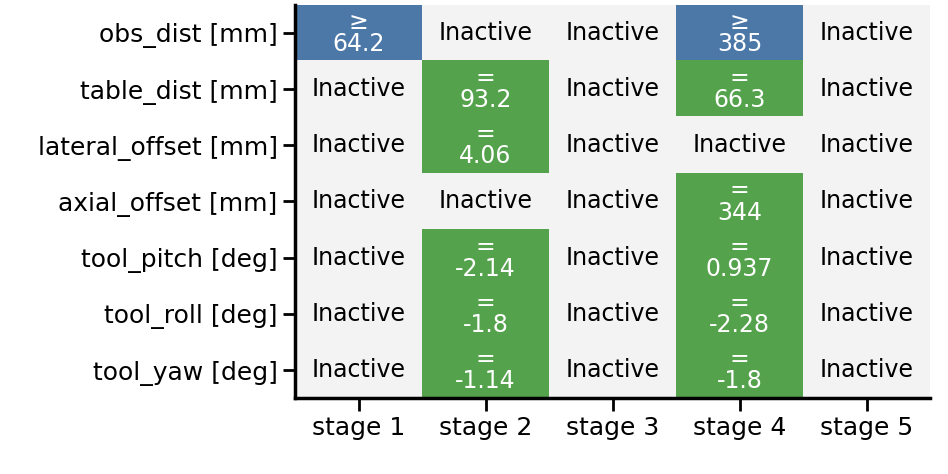
\includegraphics[width=0.86\linewidth]
    {figs/barclear_learned_constraints.png}
    \caption[Learned stage-wise constraints for the bar-clearing task.]{
    Stage-wise constraints learned for the real-robot bar-clearing task.
    }
    \label{fig:barclear_learned_constraints}
\end{figure}

\subsection{Planning and Execution}
We reuse the learned stage-wise constraint model in an optimization-based planner. For this experiment, the state $x_t\in\mathcal{X}$ is the end-effector pose expressed in a bar frame, i.e., $x_t=(p_t,R_t)$, where $p_t\in\mathbb{R}^3$ and $R_t\in SO(3)$ denote position and orientation relative to the bar. The start state, goal state and subgoals are represented in the same frame.

Let $(\widehat{\Gamma},\widehat{\mathcal{P}})$ be the constraint model recovered from the demonstrations, with learned modes $\widehat{\gamma}_{k,j}$ and parameters $\widehat{\eta}_{k,j}$. For each stage, the subgoal $g_k$ is set to the average of the corresponding stage endpoints over all demonstrations. Whereas the final subgoal is the specified terminal state, $g_K=x_{\mathrm{goal}}$. To use the learned equality and inequality constraints in a common objective, we define the violation residual
\begin{equation}
r_{k,j}(x)=
\begin{cases}
0, & \widehat{\gamma}_{k,j}=\varnothing,\\
\phi_j(x)-\widehat{\eta}_{k,j}, & \widehat{\gamma}_{k,j}=\mathrm{eq},\\
\left[\widehat{\eta}_{k,j}-\phi_j(x)\right]_+, & \widehat{\gamma}_{k,j}=\mathrm{lb},\\
\left[\phi_j(x)-\widehat{\eta}_{k,j}\right]_+, & \widehat{\gamma}_{k,j}=\mathrm{ub},
\end{cases}
\label{eq:barclear_constraint_residual}
\end{equation}
where $[z]_+=\max(z,0)$. Thus, an equality constraint is penalized according to its deviation from the learned target, while an inequality constraint incurs a penalty only on its infeasible side.

The planner discretizes each stage according to a fixed spatial waypoint spacing. If stage $k$ contains $T_k$ waypoints, its boundary is $b_k=1+\sum_{l=1}^{k}T_l$. Note that, $B$ specifies only the waypoint allocation across stages and does not prescribe their execution duration. Planning is then formulated as
\begin{equation}
\begin{aligned}
\min_{\tau=\{x_t\}_{t=1}^{T}}\quad
& J_{\mathrm{smooth}}(\tau)
+\lambda_c\sum_{k=1}^{K}\sum_{t\in\mathcal{I}_k(B)}\sum_{j=1}^{F}r_{k,j}(x_t)^2 \\
\mathrm{s.t.}\quad
& x_1=x_{\mathrm{start}},\\
& x_{b_k-1}=g_k, \qquad k=1,\dots,K,\\
& \tau\in\mathcal{C}_{\mathrm{known}}.
\end{aligned}
\label{eq:barclear_trajectory_optimization}
\end{equation}
Here, $J_{\mathrm{smooth}}$ penalizes path length and rapid changes in end-effector position and orientation, and $\lambda_c$ is a large weight penalizing constraint violation. $\mathcal{C}_{\mathrm{known}}$ specifies the known workspace limit. The problem is therefore a nonlinear optimization problem and is solved with a SciPy library.

After optimization, the task-space waypoints are converted to joint-space waypoints using sequential inverse kinematics (IK). The IK solution for each waypoint is initialized from the previous waypoint so that the resulting joint path remains on a consistent solution branch. The joint path is then time-parameterized using the average speed in each stage of the demonstrations. The generated trajectory contains joint positions, velocities, accelerations, and timestamps, and is sent to a standard ROS joint-position trajectory controller. The controller interpolates the time-parameterized joint trajectory and communicates the commands to the
robot through the position-control interface at \(200\,\mathrm{Hz}\).


\subsection{Results}
We evaluate whether the learned constraints support successful task execution on the real robot using three task-level criteria: obstacle avoidance, sweeping the objects off the bar, and sweeping the objects off the table. We varied the positions and orientations of both the obstacle and the bar and evaluated 20 execution trials. The robot passed the obstacle in 18 of 20 trials ($90\%$); the two failures were caused by excessively tilted initial tool poses. It successfully swept the objects off the bar in all 20 trials ($100\%$) and swept the objects off the table in 17 of 20 trials ($85\%$). The latter failures occurred when too many objects were placed or when the objects can easily roll away on the table.

\begin{figure*}[t]
    \centering
    \subfloat[stage 1: approach]{
        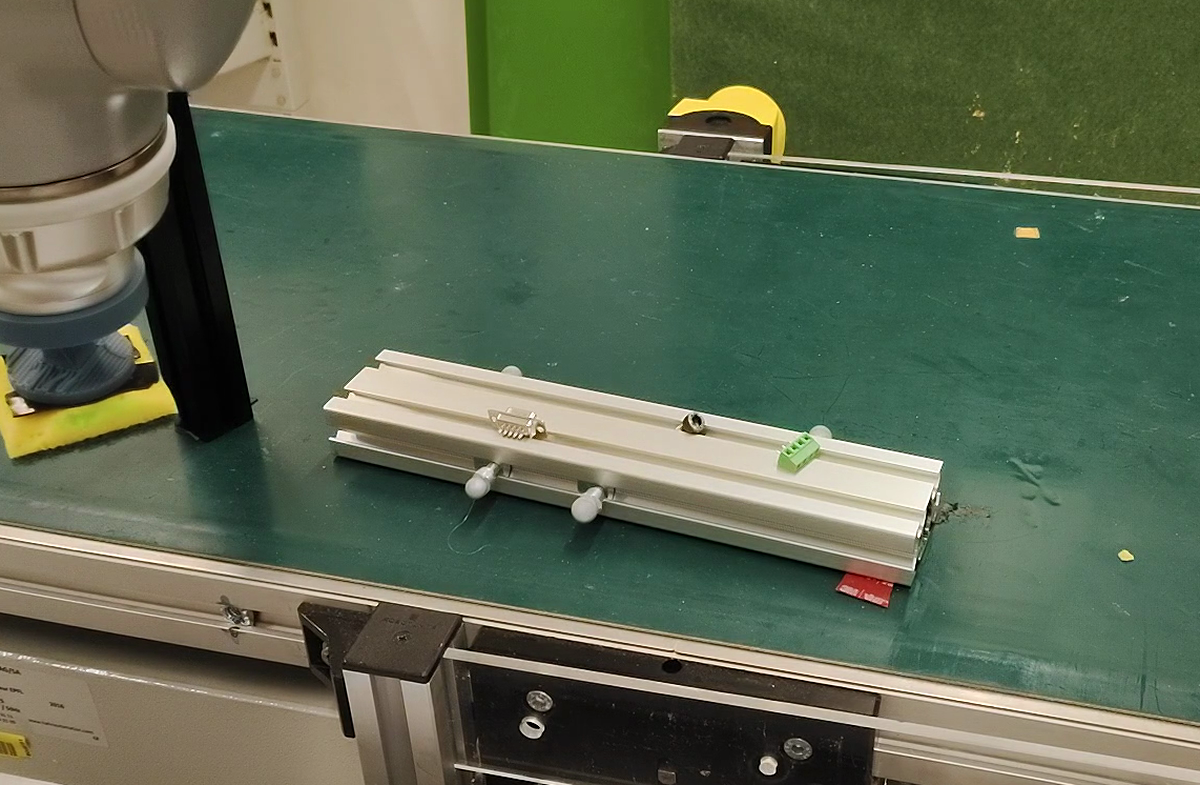
\includegraphics[width=0.235\textwidth]{figs/barclear_asss10_stage1.png}
    }\hfill
    \subfloat[stage 2: bar sweeping]{
        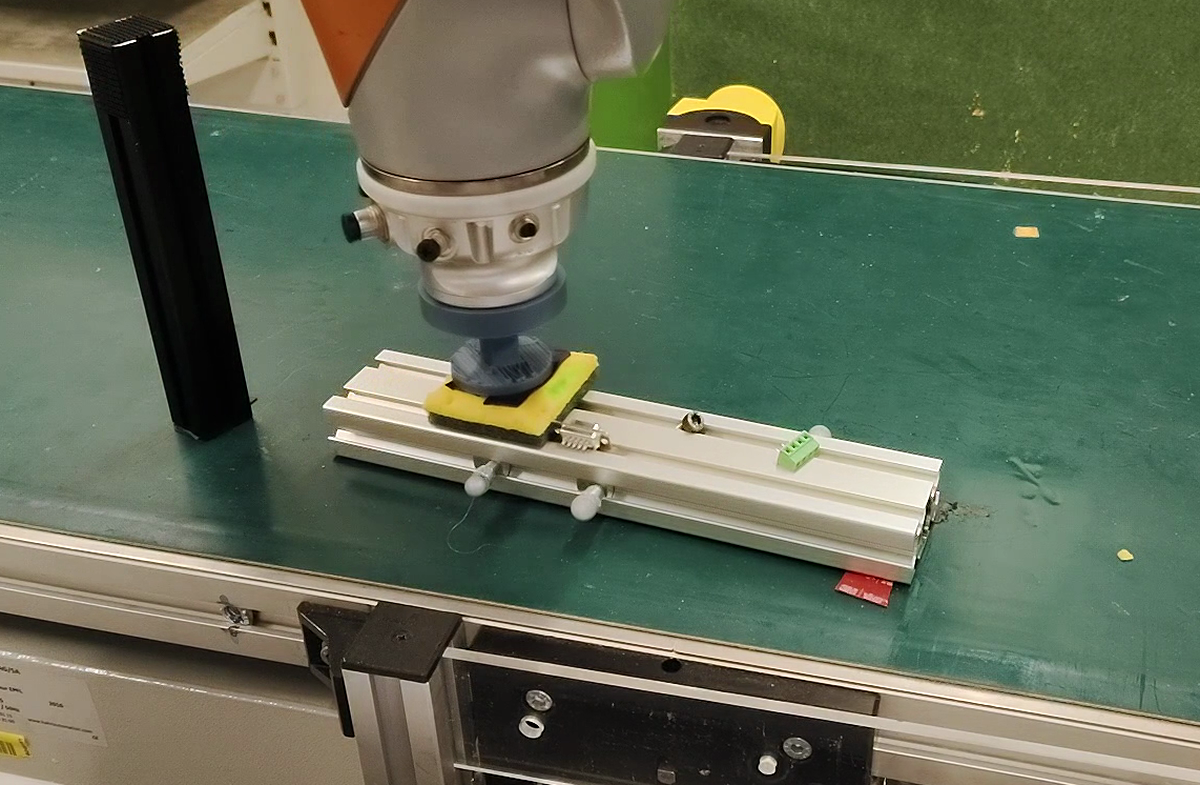
\includegraphics[width=0.235\textwidth]{figs/barclear_asss10_stage2.png}
    }\hfill
    \subfloat[stage 3: repositioning]{
        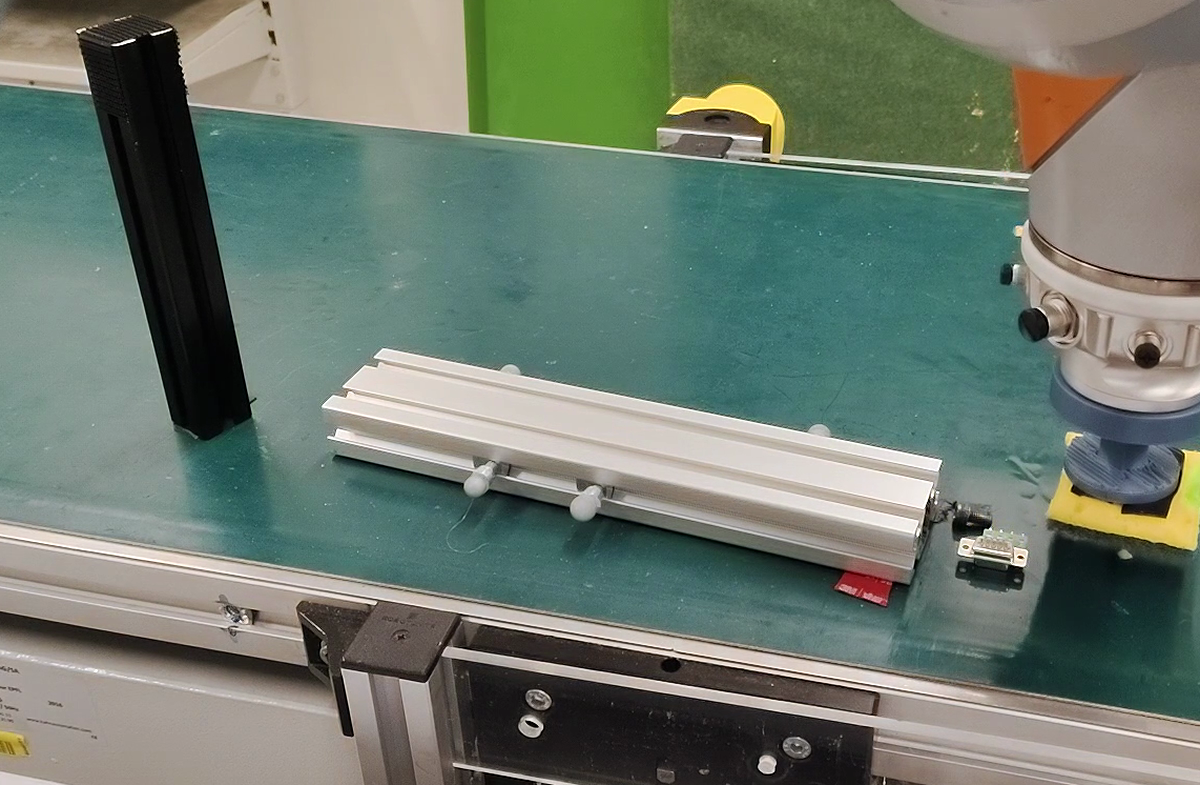
\includegraphics[width=0.235\textwidth]{figs/barclear_asss10_stage3.png}
    }\hfill
    \subfloat[Stage 4: table sweeping]{
        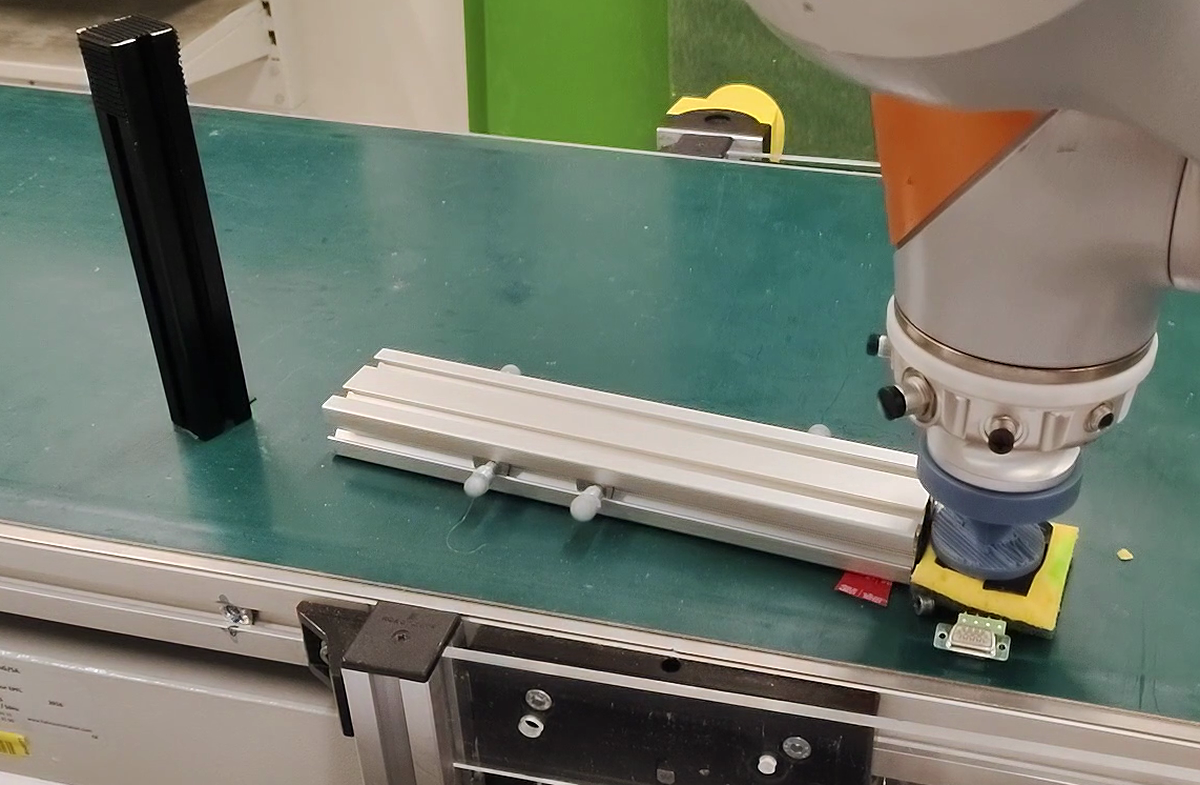
\includegraphics[width=0.235\textwidth]{figs/barclear_asss10_stage4.png}
    }
    \caption{Representative snapshots from a real-robot execution of the bar-clearing task using the learned stage-wise constraints. The four snapshots show the first four stages: (a) approaching the bar while avoiding the black obstacle; (b) sweeping the litter objects from the bar onto the table; (c) repositioning the tool between the two sweeping motions; and (d) sweeping the litter objects off the table. The final departure stage is omitted.}
    \label{fig:barclear_execution_snapshots}
\end{figure*}

The learned constraints can also be transferred to related environments. As shown in Fig.~\ref{fig:barclear_transfer}, we replace the straight bar with a curved bar and introduce an additional obstacle. The geometry of the curved bar is known and is used to compute the corresponding bar-relative features, while the learned stage-wise constraint model remains unchanged.  \texttt{obs\_dist} is evaluated with
respect to the nearest of the two obstacles. The robot successfully completes the bar-clearing task in this transferred setting and examples are provided in the video.

\begin{figure}[t]
    \centering
    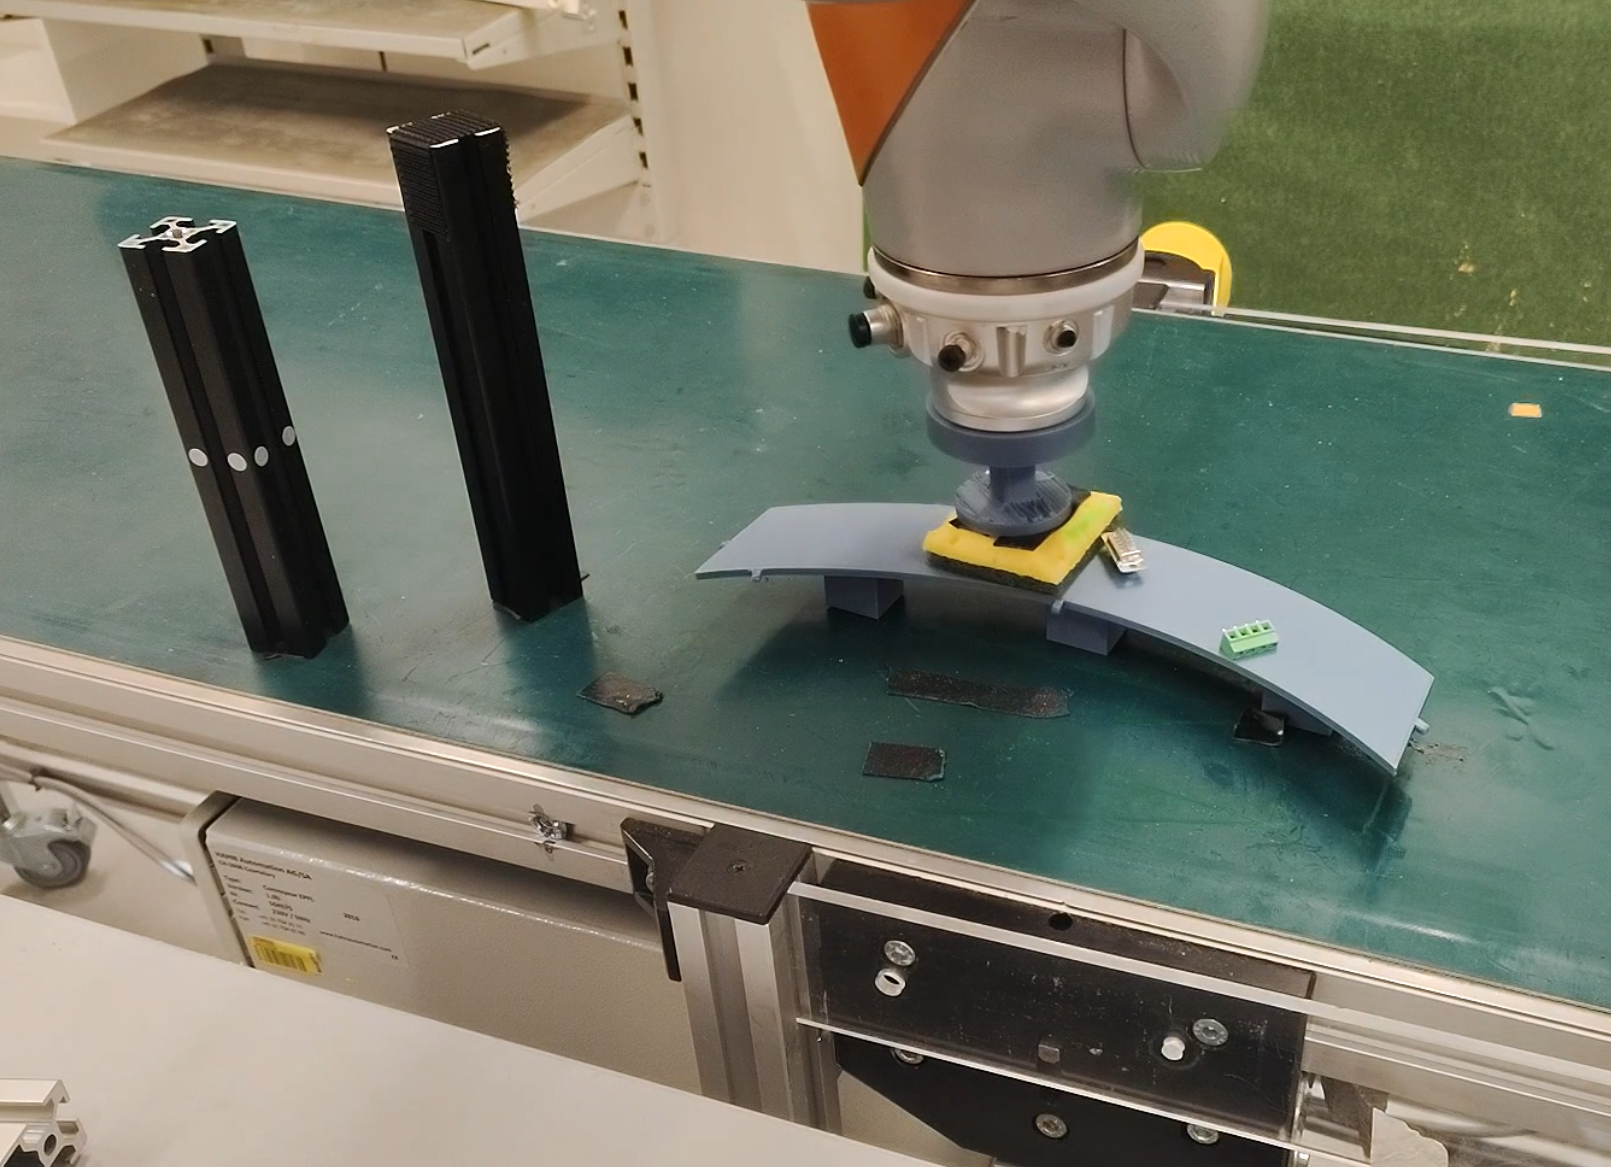
\includegraphics[width=0.58\linewidth]{figs/barclear_transfer.png}
    \caption{Transfer setting with a curved bar and an additional obstacle.}
    \label{fig:barclear_transfer}
\end{figure}

\section{Conclusion}
\label{sec:conclusion}

This paper studied stage-wise constraint learning from feasible demonstrations, where different feature constraints may become active in different stages and the stage cutpoints are unobserved. We represented the shared structure by a constraint mode matrix, whose entries indicate whether each stage-feature pair is inactive, equality-constrained, lower-bound constrained, or upper-bound constrained, together with scalar parameters for active constraints. We proposed SWCL, a method that evaluates candidate segments using local constraint evidence, subgoal-progress consistency, and cross-demonstration consensus. Conditioned on the current prototypes, each demonstration is segmented by dynamic programming, and the shared constraint modes and parameters are updated from the recovered segments.

Experiments on three simulated benchmark tasks showed that SWCL recovers more accurate stage cutpoints and constraint parameters than HMM-, HSMM-, and clustering-based baselines. The learned constraint mode matrices further show that SWCL can identify stage-dependent constraint structures across demonstrations. Planning experiments also demonstrated that the learned constraints can be reused as feasibility conditions for modified or new task instances.

The method still assumes a known number of stages. The known-stage assumption could be relaxed by allowing the dynamic-programming procedure to choose the number of stages automatically, which is an interesting direction to explore in the future. A possible extension is to add a fixed penalty for introducing each new stage: the optimizer would then create an additional segment only when the reduction in the stage-wise segmentation cost is large enough to compensate for this penalty.



\bibliographystyle{IEEEtran}
\bibliography{ref}
% \begin{thebibliography}{1}
% \bibliographystyle{IEEEtran}


\end{document}Unable to help with that. Please provide the text of the paragraph for further assistance.
